\article{同余关系与 Shimura 曲线}{Congruence relations and Shimura curves}{Yasutaka Ihara}{2}{291--311}

\origsection{}{引言（Introduction）}
关于有限域（finite field）$\F_q$ 上一维函数域（function field）$K$ 的非阿贝尔互反律（nonabelian reciprocity），已有两条研究路线。一个方向是 Drinfeld 最近优美的工作，它实现了 Langlands 思想的一部分，将 $\GL_2(K_\A)$ 的每个自守表示（automorphic representation）对应到 $K$ 上 Galois 群的一族 $l$ 进表示（$l$-adic representation）。另一条路线开展得更早，主要研究特征零的自守函数（automorphic function）。我在讲义[5b]中为这条路线提出了明确的猜想，另见[5a,c]。其目标是利用 $\operatorname{PSL}_2(\R)\times\operatorname{PGL}_2(k)$ 的离散子群（discrete subgroup）$\Gamma$，为 $\F_q$ 上代数曲线 $X$ 建立某种算术单值化理论（arithmetic uniformization），其中 $k$ 为满足 $N(\mathfrak p)=q$ 的 $\mathfrak p$ 进域。

例如，设 $p$ 为素数，$X_N$ 为 $\F_{p^2}$ 上级 $N\not\equiv0\pmod p$ 的典范模曲线（canonical modular curve）。则 $X_N$ 的全部普通闭概形点（ordinary closed scheme-theoretic point）的空间 $\mathfrak P(X_N)$ 可写成商 $\Gamma_N\backslash\mathcal H$，其中 $\Gamma_N$ 为 $\Z[1/p]$ 上级 $N$ 的模群（modular group），$\mathcal H$ 为 $M_2(\Q)$ 中满足 $(M/p)=1$ 的全部虚二次子域（imaginary quadratic subfield）$M$ 的空间。这一同时单值化
$\mathfrak P(X_N)=\Gamma_N\backslash\mathcal H$ 很重要，因为它自然描述了覆盖系统（covering system）$\{X_N/X_1\}$ 中的全部 Frobenius 元素。\footnote{§7.1简要回顾这一单值化。}这些结论的证明见[5b, 第1、2卷第5章]，其中利用了 Deuring 关于椭圆曲线约化的精妙结果；这些椭圆曲线由 $\mathcal H$ 的点参数化。[6]还给出了系统 $\{X_N/X_1\}$ 的一个简单刻画。

当前工作始于一个观察：仅以 Kronecker 同余关系（Kronecker congruence relation）$T(p)\otimes\F_p=\Pi\cup{}^t\Pi$ 为基础，就能证明上述结论。这一观察值得系统研究，理由有三。第一，由于 Shimura 的工作，Shimura 曲线对几乎所有 $p$ 也有同余关系。第二，可能存在 Shimura 曲线以外、具有非分歧同余关系的曲线。第三，同余关系本身可以作为某个范畴的对象（categorical object）。这个范畴很可能与 $\Gamma$ 所成的范畴，以及带有适当附加结构的 $X$ 所成的范畴等价；澄清这些等价关系具有重要意义。

本文概述我们关于抽象同余关系的理论。等价地说，研究对象是 CR 系统（CR-system，§1）。其主要断言是：只要 $o$ 上存在非分歧对称 CR 系统 $\mathcal X$（定义1.1.1、1.5.1），就能利用 $\operatorname{PSL}_2(\R)\times\Aut(\mathcal T)$ 的离散子群 $\Gamma$，为 $\F_q$ 上代数曲线 $X$ 建立令人满意的算术单值化理论。\footnote{AMS（MOS）主题分类（1970）：主要14G15、12A90；次要14H30、10D10。}这里 $o$ 是 $\mathfrak p$ 进域 $k$ 的整数环（$N\mathfrak p=q$），$\mathcal T$ 为与 $\operatorname{PGL}_2(k)$ 相联系的树（tree），见主定理I--III。随后将这一理论应用于 Shimura 曲线：$X$ 是其光滑约化，$\Gamma$ 则是 $\operatorname{PSL}_2(\R)\times\operatorname{PGL}_2(k)$ 中由四元数代数得到的离散子群。

§7.2讨论与其他工作的一些联系。部分证明完全省略，包括前次公告[9a]中曾给出梗概的证明。细节[9b]即将发表。

\origsection{}{记号与术语（Notations and terminologies）}
$o$：特征零、剩余域为有限域 $\F_q$ 的完备离散赋值环（complete discrete valuation ring）；$\mathfrak p$：$o$ 的极大理想；$k$：$o$ 的分式域（quotient field）；$\Spec o=\{\eta,s\}$，其中 $\eta$ 为泛点（generic point），$s$ 为闭点（closed point）。

若 $Z$ 为 $o$ 概形，$Z_\eta=Z\otimes_ok$ 表示其在 $\eta$ 上的纤维（一般纤维 general fiber），$Z_s=Z\otimes_o\F_q$ 表示其在 $s$ 上的纤维（特殊纤维 special fiber）。

对任意域 $F$，用 $\overline F$ 表示其代数闭包。若 $Z$ 为 $F$ 上固有、光滑、不可约代数曲线，则写 $\overline Z=Z\otimes_F\overline F$。若 $F'$ 为 $Z$ 的全常数域（exact constant field），则 $\overline Z$ 有 $[F':F]$ 个连通分支。$Z$ 的亏格（genus）$g$ 定义为
$g-1=[F':F](\overline g-1)$，其中 $\overline g$ 为 $\overline Z$ 各分支的亏格。

$k_d\subset\overline k$：$k$ 的唯一 $d$ 次非分歧扩张；$o_d$：$k_d$ 的整数环；$[q]$：$\bigcup_dk_d$ 在 $k$ 上的 Frobenius 自同构。

\origsection{1}{同余关系（Congruence relations）}
\paragraph*{1.1.}
设 $X$ 为 $\F_q$ 上固有、光滑、不可约代数曲线，不假设它绝对不可约（absolutely irreducible）。设 $\Pi$（分别地，${}^t\Pi$）为 $q$ 次幂态射 $X\longrightarrow X$（分别地，$X\longleftarrow X$）在 $X\times_{\F_q}X$ 上的图。将 $\Pi,{}^t\Pi,\Pi\cup{}^t\Pi$ 视为 $X\times_{\F_q}X$ 的闭约化子概形（closed reduced subscheme）。

\begin{originaltheorem}{定义 1.1.1（Definition 1.1.1）}
二维整 $o$ 概形（integral $o$-scheme）的三元组 $(X_1,X_2;T)$ 称为关于 $(X,o)$ 的同余关系，若：

(i) $X_1,X_2$ 在 $o$ 上固有且光滑，并以 $X$ 为特殊纤维；

(ii) $T$ 为 $S=X_1\times_oX_2$ 的闭子概形，在 $o$ 上平坦（flat），且
$T\times_S(X\times_{\F_q}X)=\Pi\cup{}^t\Pi$。
\end{originaltheorem}
设 $\mu:X_0\longrightarrow T$ 为二维整概形 $T$ 的正规化（normalization），令 $\varphi_i=\operatorname{pr}_i\circ\mu$（$i=1,2$），其中 $\operatorname{pr}_i$ 为 $T$ 到 $X_i$ 的投影。所得系统
\[
 \mathcal X=\{X_1\xleftarrow{\varphi_1}X_0\xrightarrow{\varphi_2}X_2\}\tag{1.1.2}
\]
称为关于 $(X,o)$ 的 CR 系统。由于 $T$ 是 $X_0$ 在 $X_1\times_oX_2$ 中的像，对应 $(X_1,X_2;T)\mapsto\mathcal X$ 是可逆的。因此同余关系与 CR 系统是两个等价的概念，下文主要采用后者。

\paragraph*{1.2.}
设 $\F_{q^c}$（$c\geq1$）为 $X$ 的全常数域。容易看出，$X_i$（$i=0,1,2$）的全常数环为 $o_c$。此外，$T$ 不可约，而 $X_1\times_oX_2$ 的连通分支与 $X\times_{\F_q}X$ 的连通分支一一对应，因此$\Pi$ 与 ${}^t\Pi$ 必须位于 $X\times_{\F_q}X$ 的同一分支中。这表明，$c=1$ 或 $c=2$。

\begin{originaltheorem}{定义 1.2.1（Definition 1.2.1）}
当 $c=1$ 时，称 $\mathcal X$ 属于情形1（Case 1）；$c=2$ 时属于情形2（Case 2）。
\end{originaltheorem}
用 $g$ 表示 $\overline X=X\otimes_{\F_q}\overline\F_q$ 的亏格。

\paragraph*{1.3.}
由定义容易得出，$X_{i\eta}=X_i\otimes_ok$（$i=0,1,2$）为 $k$ 上固有光滑不可约代数曲线。令 $\overline X_{i\eta}=X_{i\eta}\otimes_k\overline k$，用 $g_i$ 表示 $\overline X_{i\eta}$ 的亏格。则 $g_1=g_2=g$。令 $\varphi_{i\eta}=\varphi_i\otimes_ok$（$i=1,2$），则它们为次数 $q+1$ 的有限 $k$ 态射。因此 Hurwitz 公式（Hurwitz formula）给出
\[
 g_0-1=(q+1)(g-1)+\tfrac12\delta,\tag{1.3.1}
\]
其中 $\delta$ 为 $\varphi_{i\eta}$ 的不同除子（different divisor，原文德语 Differente）在 $k$ 上的次数。

\paragraph*{1.4.}
当 $x$ 遍历 $X$ 的全部 $\F_{q^2}$ 有理点时，$y=(x,x^q)$ 遍历 $T_s$ 上交集 $\Pi\cap{}^t\Pi$ 的全部几何点。将 $y$ 视为二维概形 $T$ 的点，局部环 $\mathcal O_{T,y}$ 是否正规（normal）取决于 $x$。

\begin{originaltheorem}{定义 1.4.1（Definition 1.4.1）}
若 $y=(x,x^q)$ 为 $T$ 的正规点，则称 $X$ 的 $\F_{q^2}$ 有理点 $x$ 为特殊点（special point）。记特殊点为 $x_1,\ldots,x_H$。$X$ 的其他全部 $\overline\F_q$ 有理点称为普通点（ordinary point）。
\end{originaltheorem}
$T$ 的正规化 $X_0$ 的特殊纤维 $X_{0s}$ 有两个不可约分支，经由 $\mu$ 可分别识别为 $\Pi$ 与 ${}^t\Pi$。这两个分支在满足 $x$ 为特殊点的 $y=(x,x^q)$ 上方相交。因此，由 $X_{0\eta}$ 与 $X_{0s}$ 的 Euler--Poincaré 特征（Euler--Poincaré characteristic）相同，得到
\[
 g_0-1=2(g-1)+H.\tag{1.4.2}
\]
再由(1.3.1)，得到特殊点数目的公式
\[
 H=(q-1)(g-1)+\tfrac12\delta.\tag{1.4.3}
\]
由 Zariski 连通性定理（Zariski connectedness theorem）[4, III, 4.3.1]，$H$ 总为正。

\paragraph*{1.5.}
\begin{originaltheorem}{定义 1.5.1（Definition 1.5.1）}
(i) 若 $\varphi_{1\eta},\varphi_{2\eta}$ 非分歧（unramified），则称 $\mathcal X$ 非分歧。

(ii) 若 $X_2=X_1$ 且 ${}^tT=T$，其中 ${}^tT$ 为 $T$ 的转置，则称 $\mathcal X$ 对称（symmetric）。更确切地说，存在一对互逆的 $o$ 同构 $\mathcal E_1:X_1\xrightarrow{\sim}X_2$、$\mathcal E_2:X_2\xrightarrow{\sim}X_1$，它们提升 $X$ 的恒等映射，并满足 $(\mathcal E_1\times\mathcal E_2)(T)={}^tT$。容易证明，这样的对称 $(\mathcal E_1,\mathcal E_2)$ 若存在便唯一，见[9b, §1]。
\end{originaltheorem}
由(1.4.3)，$\mathcal X$ 非分歧时有 $H=(q-1)(g-1)$，反之亦然。特别地，$\mathcal X$ 非分歧时 $g>1$。

\paragraph*{1.6.}
当 $o=\Z_p$ 为 $p$ 进整数环时，可应用我们先前的工作[10]，证明下述非分歧同余关系的刚性（rigidity）。
\begin{originaltheorem}{定理 1.6.1（Theorem 1.6.1）}
给定 $X$ 及 $X$ 的 $\F_{p^2}$ 有理点的集合 $\mathfrak S$。则关于 $(X,\Z_p)$、以 $\mathfrak S$ 为特殊点集合的非分歧 CR 系统 $\mathcal X$ 至多唯一。且若存在，它必对称。
\end{originaltheorem}
所以，当 $o=\Z_p$ 时，非分歧蕴含对称。存在性问题更难。我们已经知道 $\mathcal X$ 存在的必要条件 $|\mathfrak S|=(q-1)(g-1)$，但这并不充分。这一问题实质上与 $X$ 的形式提升（formal lifting）上的一个微分形式有关，见[10]、[7]。我希望在不久将来讨论[10]的进一步发展。

\paragraph*{1.7.}
最熟知的同余关系是 Kronecker 同余关系 $(X_1,X_2;T)$，其中 $X_1=X_2$ 为 $\Z_p$ 上射影 $j$ 直线，$T$ 为由 $p$ 阶模方程（modular equation）$\Phi_p(j,j')=0$ 定义的 $X_1\times_{\Z_p}X_2$ 的闭子概形。这个 CR 系统是对称的，并且存在分歧。众所周知，除同样为普通点的尖点之外，普通点（分别地，特殊点）为 $\overline\F_p$ 上椭圆曲线的奇异（singular，原文如此）（分别地，超奇异 supersingular）$j$ 不变量。其他例子见§6及[9a]。

\origsection{2}{第一 Galois 理论（The first Galois theory）}
设 $\mathcal X=\{X_1\xleftarrow{\varphi_1}X_0\xrightarrow{\varphi_2}X_2\}$ 为任意关于 $(X,o)$ 的 CR 系统。本节研究以下 $k$ 上的系统：
\[
 \mathcal X_\eta=\{X_{1\eta}\xleftarrow{\varphi_{1\eta}}
 X_{0\eta}\xrightarrow{\varphi_{2\eta}}X_{2\eta}\}
\]
并建立它的一项基本 Galois 理论性质，为后文作准备。

\paragraph*{2.1.}
用 $K_i$ 表示 $X_i$（$i=0,1,2$）的函数域。则每个 $K_i$ 都是全常数域为 $k_c$ 的一元代数函数域（参见§1.2）。态射 $\varphi_i$（$i=1,2$）诱导嵌入 $K_i\hookrightarrow K_0$，且 $K_0=K_1K_2$、$[K_0:K_i]=q+1$。

\begin{originaltheorem}{定义 2.1.1（Definition 2.1.1）}
$L$ 为 $K_0$ 的最小 Galois 扩张，使 $L/K_1$、$L/K_2$ 都是 Galois 扩张。
\end{originaltheorem}
记 $V_i=\Gal(L/K_i)$（$i=0,1,2$），注意 $V_0=V_1\cap V_2$。
\begin{originaltheorem}{定义 2.1.2（Definition 2.1.2）}
$G_{\mathfrak p}^+$ 为 $\Aut(L/k)$ 中由 $V_1,V_2$ 生成的子群。
\end{originaltheorem}
将 $V_i$ 的 Krull 拓扑（Krull topology）扩张为 $G_{\mathfrak p}^+$ 的拓扑，以“$V_i$ 为开子群”刻画之。

\paragraph*{2.2.}
暂假设 $\mathcal X$ 为 Kronecker CR 系统（§1.7）。在通常记号下，$K_1=\Q_p(j(\tau))$、$K_2=\Q_p(j(p\tau))$，$L$ 为在 $\Q_p$ 上由全部形如 $j(p^n\tau+b)$（$n\in\Z$、$b\in\Z[1/p]$）的函数生成的域。这表明
\[
 V_1=\operatorname{PGL}_2(\Z_p),\qquad
 V_2=\begin{pmatrix}0&-1\\p&0\end{pmatrix}^{-1}
 V_1\begin{pmatrix}0&-1\\p&0\end{pmatrix},
\]
而 $G_{\mathfrak p}^+=\operatorname{PGL}_2^+(\Q_p)$，这里一般地
\[
 \operatorname{PGL}_2^+(k)=
 \{g\in\GL_2(k):\operatorname{ord}_{\mathfrak p}\det g\equiv0\pmod2\}/k^\times.
\]
此时，$G_{\mathfrak p}^+$ 相对于 $V_1,V_2$ 的结构是已知的。由相应双陪集环（double coset ring）的结构可知， $G_{\mathfrak p}^+$ 为 $V_1,V_2$ 关于公共子群 $V_0$ 的融合自由积（free product with amalgamation），见[5b, 第1卷第2章§28]、[16]。我们能证明，这些都是同余关系的一般现象。

\paragraph*{2.3.}
更确切地说，对任意 CR 系统 $\mathcal X$，将两个左陪集空间的不交并
$(V_1\backslash G_{\mathfrak p}^+)\sqcup(V_2\backslash G_{\mathfrak p}^+)$ 视为点集，记为 $\mathcal T^0$。若属于不同陪集空间的两点 $V_1g,V_2g'$ 满足 $V_1g\cap V_2g'\ne\varnothing$，则称它们相邻（mates）。由于 $(V_i:V_0)=q+1$，每点恰有 $q+1$ 个相邻点。将点集 $\mathcal T^0$ 中每对相邻点以线段连接，得到图
$\mathcal T=\mathcal T(G_{\mathfrak p}^+;V_1,V_2)$。$G_{\mathfrak p}^+$ 通过右乘作用于 $\mathcal T$；由 $L$ 的最小性，作用忠实（effective）。

\begin{originaltheorem}{定理 2.3.1（Theorem 2.3.1）}
设 $\mathcal X$ 为任意 CR 系统，令 $\mathcal T=\mathcal T(G_{\mathfrak p}^+;V_1,V_2)$。则(i) $\mathcal T$ 连通且无圈（acyclic）；换言之，对任意点 $A,B\in\mathcal T^0$，存在一个
% 原书第295页；来源：用户补充截图 source-supplements/volume-2-p295.png。
唯一点列 $A=A_0,A_1,\ldots,A_l=B$，使得对 $0\leq i\leq l-1$，$A_i,A_{i+1}$ 相邻，且对 $1\leq i\leq l-1$，有 $A_{i-1}\ne A_{i+1}$。记 $l=l(A,B)$，称为 $A,B$ 之间的长度（length）。

(ii) 若 $A,B,A',B'\in\mathcal T^0$ 满足 $l(A,B)=l(A',B')$，且 $A,A'$ 属于同一陪集空间 $V_1\backslash G_{\mathfrak p}^+$ 或 $V_2\backslash G_{\mathfrak p}^+$，则存在 $g\in G_{\mathfrak p}^+$，使 $A'=A^g$、$B'=B^g$。
\end{originaltheorem}

特别地，$\mathcal T^0$ 为无限集，因此 $(G_{\mathfrak p}^+:V_0)=\infty$。此外，由(ii)得到 $(V_0:\{1\})=\infty$，即 $[L:K_0]=\infty$。这特别蕴含 $K_1\cap K_2=k_c$。由(i)直接得到：

\begin{originaltheorem}{推论 2.3.2（Corollary 2.3.2）}
$G_{\mathfrak p}^+$ 是 $V_1,V_2$ 关于公共子群 $V_0$ 的融合自由积。
\end{originaltheorem}

\paragraph*{2.4.}
$\mathcal T$ 的图形如下（$q=2$）：
\begin{center}
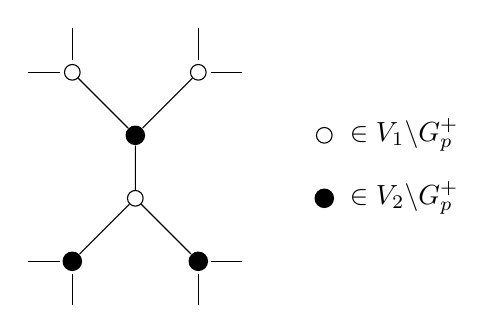
\begin{tikzpicture}[scale=.8]
 \node[circle,draw,inner sep=2pt] (a) at (-1,1.5) {};
 \node[circle,draw,inner sep=2pt] (b) at (1,1.5) {};
 \node[circle,fill=black,inner sep=2.5pt] (c) at (0,.5) {};
 \node[circle,draw,inner sep=2pt] (d) at (0,-.5) {};
 \node[circle,fill=black,inner sep=2.5pt] (e) at (-1,-1.5) {};
 \node[circle,fill=black,inner sep=2.5pt] (f) at (1,-1.5) {};
 \draw (a)--(c)--(b) (c)--(d)--(e) (d)--(f);
 \draw (-1,1.7)--(-1,2.2) (-1.2,1.5)--(-1.7,1.5)
       (1,1.7)--(1,2.2) (1.2,1.5)--(1.7,1.5)
       (-1,-1.7)--(-1,-2.2) (-1.2,-1.5)--(-1.7,-1.5)
       (1,-1.7)--(1,-2.2) (1.2,-1.5)--(1.7,-1.5);
 \node[circle,draw,inner sep=2pt] at (3,.5) {};
 \node[anchor=west] at (3.25,.5) {$\in V_1\backslash G_{\mathfrak p}^+$};
 \node[circle,fill=black,inner sep=2.5pt] at (3,-.5) {};
 \node[anchor=west] at (3.25,-.5) {$\in V_2\backslash G_{\mathfrak p}^+$};
\end{tikzpicture}\qquad(2.4.1)
\end{center}
这正是与群 $\operatorname{PGL}_2(k)$ 对应的树。

\paragraph*{注 2.4.2.}
群 $G_{\mathfrak p}^+$ 与 $\operatorname{PGL}_2^+(k)$ 忠实作用于“同一个”图 $\mathcal T$，而且顶点轨道相同，分别为空心顶点和实心顶点。已有例子表明，若不对 $\mathcal X$ 施加非分歧等条件，$G_{\mathfrak p}^+$ 可以严格大于 $\operatorname{PGL}_2^+(k)$。

\paragraph*{2.5.}
定理2.3.1的证明只基于下述事实：“存在 $K_1$ 的离散赋值 $v_1$、$K_2$ 的离散赋值 $v_2$，及 $K_0$ 的离散赋值 $w_1,w_2$，满足：(a) 对每个 $i=1,2$，$w_1,w_2$ 为 $v_i$ 到 $K_0$ 的全部不同延拓；(b) 对每个 $i=1,2$，$K_i$ 在 $K_0$ 中关于 $w_i$ 进拓扑稠密。”局部环 $\mathcal O_{X_i,X_{is}}$、$\mathcal O_{X_0,\Pi}$、$\mathcal O_{X_0,{}^t\Pi}$ 定义了具有这些性质的赋值 $v_i,w_1,w_2$。

\paragraph*{2.6.}
令 $\overline k\cap L$ 为 $k$ 在 $L$ 中的代数闭包。$G_{\mathfrak p}^+$ 作用于 $\overline k\cap L$，且不动域为 $k_c$。因此 $(\overline k\cap L)/k_c$ 为 Galois 扩张。若用 $\overline{G_{\mathfrak p}^+}$ 表示 $G_{\mathfrak p}^+$ 在 $\overline k\cap L$ 上作用的核，则有典范同构
\[
 \Aut((\overline k\cap L)/k_c)
 \simeq G_{\mathfrak p}^+/\overline{G_{\mathfrak p}^+}.
\]
关于 $\overline k\cap L$ 的“大小”，以下断言已经足够。

\begin{originaltheorem}{命题 2.6.1（Proposition 2.6.1）}
对任意 $g,g'\in G_{\mathfrak p}^+$ 及 $1\leq i,j\leq2$，$k_c$ 在 $K_i^g\cdot K_j^{g'}$ 中代数闭；换言之，
\[
 G_{\mathfrak p}^+
 =\bigl[(g^{-1}V_ig)\cap((g')^{-1}V_jg')\bigr]
 \cdot\overline{G_{\mathfrak p}^+}.
\]
\end{originaltheorem}
利用上述赋值 $v_i,w_i$ 的基本性质，容易证明此命题。

\paragraph*{2.7.}
当 $\mathcal X$ 对称时，等式 $X_2=X_1$ 定义同构 $K_1\xrightarrow{\sim}K_2$；由于 ${}^tT=T$，此同构唯一扩张为 $K_0$ 的一个对合，记为 $\iota$。在情形2中，$\iota$ 在 $k_2/k$ 上诱导一个对合。由 $L$ 的定义，$\iota$ 可延拓为 $L$ 的自同构，仍

记为 $\iota$。则 $V_0\iota$ 良定义，$\iota^{-1}V_0\iota=V_0$、$\iota^2\in V_0$，且
$\iota^{-1}V_1\iota=V_2$、$\iota^{-1}V_2\iota=V_1$。

\begin{originaltheorem}{定义 2.7.1（Definition 2.7.1）}
当 $\mathcal X$ 对称时，$G_{\mathfrak p}$ 为由 $G_{\mathfrak p}^+$ 与 $\iota$ 生成的群。
\end{originaltheorem}
注意 $G_{\mathfrak p}$ 由 $V_1,\iota$ 生成，且 $(G_{\mathfrak p}:G_{\mathfrak p}^+)=2$。通过
$V_1g\leftrightarrow V_1g$、$V_2g\leftrightarrow V_1\iota g$（$g\in G_{\mathfrak p}^+$），将 $(V_1\backslash G_{\mathfrak p}^+)\sqcup(V_2\backslash G_{\mathfrak p}^+)$ 与 $V_1\backslash G_{\mathfrak p}$ 等同。因此，$V_1g,V_1g'$ 相邻，当且仅当 $g'g^{-1}\in V_1\iota V_1$。群 $G_{\mathfrak p}$ 忠实作用于 $\mathcal T$，且定理2.3.1(ii)可改写为：

(ii*) 若 $A,B,A',B'\in\mathcal T^0$ 满足 $l(A,B)=l(A',B')$，则存在 $g\in G_{\mathfrak p}$，使 $A'=Ag$、$B'=Bg$。

由定理2.3.1(i)得到：
\begin{originaltheorem}{推论 2.7.2（Corollary 2.7.2）}
$G_{\mathfrak p}$ 是 $V_1$ 与 $V_0\cup V_0\iota$ 关于公共子群 $V_0$ 的融合自由积。
\end{originaltheorem}
当 $\mathcal X$ 为 Kronecker CR 系统时，对适当延拓 $\iota$ 有
\[
 G_{\mathfrak p}=\operatorname{PGL}_2(\Q_p),\qquad
 \iota=\begin{pmatrix}0&-1\\p&0\end{pmatrix}.
\]

\paragraph*{2.8.}
回到任意 CR 系统 $\mathcal X$。若其非分歧，则 $K_0/K_1$、$K_0/K_2$ 是代数函数域的非分歧扩张，因此 $L/K_0$ 也非分歧。
\begin{originaltheorem}{定义 2.8.1（Definition 2.8.1）}
若 $K_0/k$ 的几乎所有素除子（prime divisor）在 $L$ 中非分歧，则称 $\mathcal X$ 几乎非分歧（almost unramified）。
\end{originaltheorem}
由上述说明，非分歧蕴含几乎非分歧。我不知道当 $o=\Z_p$ 时，几乎非分歧是否也蕴含对称。几乎非分歧这一条件刻画了与自守函数有关的一类 CR 系统。存在不是几乎非分歧的 $\mathcal X$ 的例子。

\paragraph*{2.9. 算术基本群（arithmetic fundamental group）$\Gamma$.}
设 $\mathcal X$ 几乎非分歧且对称。对每个 $\mathcal X$ 及嵌入 $\epsilon:k\hookrightarrow\C$（$\C$ 为复数域），可按以下方法赋予一个在共轭意义下确定的离散子群 $\Gamma\subset$
\[
 \operatorname{PSL}_2(\R)\times G_{\mathfrak p}.\tag{2.9.1}
\]
考虑 $L$ 到 $\C\cup\{\infty\}$ 的满足下述条件的全部位（place）$\xi_\C$ 的集合 $\Sigma$：(i) $\xi_\C$ 延拓 $\epsilon$；(ii) $\xi_\C$ 的赋值环或为 $L$ 本身，或为离散赋值环。令 $G_{\mathfrak p}$ 通过
$\xi_\C\mapsto g\xi_\C$ 作用于 $\Sigma$，其中
$(g\xi_\C)(a)=\xi_\C(a^g)$（$\xi_\C\in\Sigma$、$g\in G_{\mathfrak p}$、$a\in L$）。则 $\Sigma$ 带有自然的 $G_{\mathfrak p}$ 不变复结构，参见[5b, 第1卷第2章]或[9b]。此外，$\Sigma$ 的每个连通分支 $\Sigma_0$ 同构于复上半平面（complex upper half-plane）$\mathfrak H$，且 $G_{\mathfrak p}$ 在全体连通分支上可迁（transitive）。选取任意连通分支 $\Sigma_0$，令
\[
 \Gamma=\{\gamma\in G_{\mathfrak p}:\gamma\Sigma_0=\Sigma_0\}.\tag{2.9.2}
\]
则 $\Gamma$ 忠实作用于 $\Sigma_0\simeq\mathfrak H$，因而可视为 $\Aut(\mathfrak H)\simeq\operatorname{PSL}_2(\R)$ 的子群。另一方面，$\Gamma$ 自然为 $G_{\mathfrak p}$ 的子群。通过这两个嵌入，今后将 $\Gamma$ 视为 $\operatorname{PSL}_2(\R)\times G_{\mathfrak p}$ 的子群。它在该积群中的共轭类与 $\Sigma_0$ 及上述两个同构的选取无关，但实质上依赖于嵌入 $\epsilon$。

\begin{originaltheorem}{定义 2.9.3（Definition 2.9.3）}
称 $\Gamma$ 为属于 $\mathcal X,\epsilon$ 的算术基本群。
\end{originaltheorem}
令
\[
 \Gamma^+=\Gamma\cap(\operatorname{PSL}_2(\R)\times G_{\mathfrak p}^+),\qquad
 \Delta_i=\Gamma\cap(\operatorname{PSL}_2(\R)\times V_i)
 \quad(i=1,0,2).\tag{2.9.4}
\]
$\Delta_i$ 到 $\operatorname{PSL}_2(\R)$ 的投影为第一类 Fuchs 群（Fuchsian group of the first kind），当 $\mathcal X$ 非分歧时，它们正是 $X_{i\eta}\otimes_{k_c}\C$ 的泛覆盖群（universal covering group）。\footnote{当 $c=2$ 时，张量积使用 $\Sigma_0$ 所确定的嵌入 $k_c\hookrightarrow\C$。}因此 $\Gamma^+$ 在积群(2.9.1)中离散；又由下面2.9.6可知，$\mathcal X$ 非分歧时它无挠（torsion-free）。同理，积群(2.9.1)模去 $\Gamma^+$ 的商具有有限不变体积，且当 $\mathcal X$ 非分歧时紧。$\Gamma^+$ 在 $\operatorname{PSL}_2(\R)$ 中的投影稠密，在 $G_{\mathfrak p}^+$ 中的投影也稠密。

再考虑 $\Gamma$ 自身。情形2中，$\iota$ 作为 $k_2/k_1$ 的对合，故 $\Gamma=\Gamma^+$。情形1中，$K_0$ 的对称 $\iota$ 可延拓为 $\Gamma$ 的元素，仍记为 $\iota$。此时 $\Delta_0\iota$ 良定义，且
\[
 \iota^{-1}\Delta_0\iota=\Delta_0,\quad\iota^2\in\Delta_0;\qquad
 \iota^{-1}\Delta_1\iota=\Delta_2,\quad
 \iota^{-1}\Delta_2\iota=\Delta_1.\tag{2.9.5}
\]
所以 $\Gamma$ 由 $\Gamma^+,\iota$ 生成。因为 $G_{\mathfrak p}^+=V_0\Gamma^+$，且在情形1中 $G_{\mathfrak p}=V_0\Gamma$，由2.3.2、2.7.2立即得到：
\begin{originaltheorem}{推论 2.9.6（Corollary 2.9.6）}
(i) $\Gamma^+$ 为 $\Delta_1,\Delta_2$ 关于公共子群 $\Delta_0$ 的融合自由积。

(ii) 情形2中，$\Gamma=\Gamma^+$；情形1中，$\Gamma$ 为 $\Delta_1$ 与 $\Delta_0\cup\Delta_0\iota$ 关于公共子群 $\Delta_0$ 的融合自由积。
\end{originaltheorem}
当 $\mathcal X$ 为 Kronecker CR 系统时，在相差 $\operatorname{PSL}_2(\R)\times\operatorname{PGL}_2(\Q_p)$ 中共轭的意义下，
\[
 \Delta_1=\operatorname{PSL}_2(\Z),\qquad
 \Delta_2=\begin{pmatrix}0&-1\\p&0\end{pmatrix}^{-1}
 \Delta_1\begin{pmatrix}0&-1\\p&0\end{pmatrix},
\]
\[
 \Gamma^+=\operatorname{PSL}_2(\Z[1/p]),\qquad
 \Gamma=\{\gamma\in\GL_2(\Z[1/p]):\det\gamma\in p^\Z\}/\{\pm p^\Z\}.
\]

\origsection{3}{典范提升（The canonical liftings）}
设 $\mathcal X=\{X_1\xleftarrow{\varphi_1}X_0\xrightarrow{\varphi_2}X_2\}$ 为关于 $(X,o)$ 的任意 CR 系统。我们将详细研究 $L/k$ 的某类特殊位 $\xi$ 的模 $\mathfrak p$ 约化。具体来说，考虑在 $G_{\mathfrak p}^+$ 中具有“大”稳定子群的位 $\xi$；精确定义见§3.3的条件[A]。主要目标是概述定理3.4.1的证明：模 $\mathfrak p$ 约化在这些 $\xi$ 的全部 $G_{\mathfrak p}^+$ 轨道与 $X\otimes\F_{q^2}$ 的全部普通闭概形点之间诱导双射。方法是将 $X$ 的每个普通几何点 $x$ 典范提升为 $X_{i\eta}$ 的几何点 $\xi_i$（$i=1,2$）。当 $\mathcal X$ 非分歧且对称时，主要结果用 $\Gamma$ 重新表述于§3.14（主定理I）及§3.15。

\paragraph*{3.1. $\operatorname{Pl}(L/k)$ 中 $G_{\mathfrak p}^+$ 轨道的约化.}
以 $\operatorname{Pl}(L/k)$ 表示 $L$ 到 $\overline k\cup\{\infty\}$ 的所有 $k$ 位。令 $\Aut(L/k)$ 以 $\xi\mapsto g\xi$ 作用，其中 $(g\xi)(a)=\xi(a^g)$。对 $\xi\in\operatorname{Pl}(L/k)$，用 $\xi_i$ 表示它在 $K_i$ 上的限制，视为 $\overline X_{i\eta}$ 的点；用 $\xi_{is}$ 表示 $\xi_i$ 在 $\overline X$ 上的唯一特化（specialization）。因为 $T\otimes_o\F_q=\Pi\cup{}^t\Pi$，有 $\xi_{2s}=\xi_{1s}^{q^{\pm1}}$。由于 $G_{\mathfrak p}^+$ 由 $V_1,V_2$ 生成，重复应用此事实可知，对 $g\in G_{\mathfrak p}^+$ 及 $1\leq i,j\leq2$，$(g\xi)_{is}$ 与 $\xi_{js}$ 在 $\F_q$ 上共轭；当 $i=j$ 时，它们在 $\F_{q^2}$ 上共轭。当 $\mathcal X$ 对称时，对任意 $g\in G_{\mathfrak p}$，$(g\xi)_{is}$ 与 $\xi_{js}$ 均在 $\F_q$ 上共轭。注意由 $\xi\mapsto\xi_{is}$（$i=1,2$）诱导的映射：
\[
 \operatorname{Pl}(L/k)\longrightarrow\{\overline X\text{ 的点}\},\tag{$3.1.1_i$}
\]
\[
 G_{\mathfrak p}^+\backslash\operatorname{Pl}(L/k)
 \longrightarrow\{\overline X\text{ 的点的 }\F_{q^2}\text{ 共轭类}\},\tag{$3.1.2_i$}
\]
以及当 $\mathcal X$ 对称时的
\[
 G_{\mathfrak p}\backslash\operatorname{Pl}(L/k)
 \longrightarrow\{\overline X\text{ 的点的 }\F_q\text{ 共轭类}\}.\tag{$3.1.3_{\mathrm{symm}}$}
\]
两个(3.1.2)$_i$ 在 $\F_{q^2}/\F_q$ 的对合下相互变换。

\paragraph*{3.2.}
对每个 $\xi\in\operatorname{Pl}(L/k)$，定义其（超越）分解群 $D_\xi^+$ 与惯性群 $I_\xi^+$：
\[
\begin{aligned}
 D_\xi^+&=\{g\in G_{\mathfrak p}^+:g\xi\sim\xi\}
 =\{g\in G_{\mathfrak p}^+:\mathcal O_\xi^g=\mathcal O_\xi\},\\
 I_\xi^+&=\{g\in G_{\mathfrak p}^+:g\xi=\xi\}
 =\{g\in D_\xi^+:g\text{ 在 }\mathcal O_\xi/\mathfrak m_\xi\text{ 上平凡作用}\}.
\end{aligned}\tag{3.2.1}
\]
这里 $\sim$ 为位的等价关系，$\mathcal O_\xi$ 为 $\xi$ 的赋值环，$\mathfrak m_\xi$ 为其极大理想。$\mathcal X$ 对称时，同样定义 $D_\xi,I_\xi$，即删去(3.2.1)中的 $+$。显然，$I_\xi^+$（分别地 $I_\xi$）在 $D_\xi^+$（分别地 $D_\xi$）中正规。对 $g\in G_{\mathfrak p}^+$（或 $\mathcal X$ 对称时的 $g\in G_{\mathfrak p}$），定义其次数（degree）
\[
 \operatorname{Deg}(g)=\min_{A\in\mathcal T^0}l(A,A^g).\tag{3.2.2}
\]
$\operatorname{Deg}(g)$ 为非负整数，它为偶数当且仅当 $g\in G_{\mathfrak p}^+$。此外，$\operatorname{Deg}(g)=0$ 当且仅当 $g$ 在 $G_{\mathfrak p}^+$ 中共轭于 $V_1$ 或 $V_2$ 的某元素。令
\[
 I_\xi^0=\{g\in I_\xi^+:\operatorname{Deg}(g)=0\}.\tag{3.2.3}
\]

\paragraph*{3.3.}
对 $\xi\in\operatorname{Pl}(L/k)$，考虑条件：

[A] $I_\xi^0$ 构成 $I_\xi^+$ 的无限指数子群。

若 $\xi$ 满足[A]，则 $g\xi$ 也满足，其中 $g\in G_{\mathfrak p}^+$（分别地，$G_{\mathfrak p}$）。当 $\mathcal X$ 非分歧时，$L/K_i^g$（$g\in G_{\mathfrak p}^+$）非分歧，所以通常的惯性群 $I_\xi^+\cap g^{-1}V_ig$ 平凡。因此 $I_\xi^0=\{1\}$，条件[A]等价于：

[A]（$\mathcal X$ 非分歧）$I_\xi^+$ 为无限群。

回到一般 $\mathcal X$，将满足[A]的全部 $\xi$ 组成的集合记为 $\operatorname{Pl}(L/k;[A])$。它在 $G_{\mathfrak p}^+$（分别地 $G_{\mathfrak p}$）下稳定。对其中每个 $\xi$，令 $\operatorname{Deg}^+(\xi)$（当 $\mathcal X$ 对称时，分别令 $\operatorname{Deg}(\xi)$）为 $g$ 遍历 $I_\xi^+-I_\xi^0$（分别地 $I_\xi-I_\xi^0$）时 $\operatorname{Deg}(g)$ 的最小值。则 $\operatorname{Deg}^+(\xi)$ 只依赖于 $G_{\mathfrak p}^+\xi$；$\mathcal X$ 对称时，两个次数均只依赖于 $G_{\mathfrak p}\xi$。

\paragraph*{3.4.}
下面先给出§3的一项主要结果，典范提升的显式构造将在后文展开。
\begin{originaltheorem}{定理 3.4.1（Theorem 3.4.1）}
(i) 对每个 $i=1,2$，约化映射 $\xi\mapsto\xi_{is}$ 在 $\operatorname{Pl}(L/k;[A])$ 的全部 $G_{\mathfrak p}^+$ 轨道与 $\overline X$ 的普通点（§1.4）的全部 $\F_{q^2}$ 共轭类之间诱导双射，即
\[
 \operatorname{red}_i:G_{\mathfrak p}^+\backslash\operatorname{Pl}(L/k;[A])
 \xrightarrow{\sim}\{X\otimes_{\F_q}\F_{q^2}\text{ 的普通闭点}\}.
\]
且 $\operatorname{Deg}^+(\xi)=2\operatorname{Deg}(\xi_{is}/\F_{q^2})$。

(ii) 若 $\mathcal X$ 对称，$\operatorname{red}_i$（$i=1,2$）在全部 $G_{\mathfrak p}$ 轨道与 $\overline X$ 普通点的全部 $\F_q$ 共轭类之间诱导同一个双射，即
\[
 \operatorname{red}_i:G_{\mathfrak p}\backslash\operatorname{Pl}(L/k;[A])
 \xrightarrow{\sim}\{X\text{ 的普通闭点}\}.
\]
且 $\operatorname{Deg}(\xi)=\operatorname{Deg}(\xi_{is}/\F_q)$。

(iii) 对任意 $\xi\in\operatorname{Pl}(L/k;[A])$，$I_\xi^0$ 是 $I_\xi^+$ 的正规子群，且 $I_\xi^+/I_\xi^0\simeq\Z$；$D_\xi^+/I_\xi^+$ 典范同构于 $\mathcal O_\xi/\mathfrak m_\xi$ 在 $k_2\cap(\mathcal O_\xi/\mathfrak m_\xi)$ 上的完整 Galois 群。若 $\mathcal X$ 对称，则 $I_\xi^0$ 也在 $I_\xi$ 中正规，$I_\xi/I_\xi^0\simeq\Z$，且 $D_\xi/I_\xi$ 典范同构于 $\mathcal O_\xi/\mathfrak m_\xi$ 在 $k$ 上的完整 Galois 群。
\end{originaltheorem}
证明将在§3余下部分概述。关键是构造逆映射 $\xi_{is}\mapsto\xi$，将 $\xi_{is}$ 提升为满足[A]的 $\xi$（§§3.10--3.11）。先作一些准备。

\paragraph*{3.5. 树 $\mathcal T$ 上的河流（Rivers）.}
为分析 $\xi_{is}$ 为普通点时的 $G_{\mathfrak p}^+$ 轨道，引入树 $\mathcal T=\mathcal T(G_{\mathfrak p}^+;V_1,V_2)$ 上的“河流”概念。
\begin{originaltheorem}{定义 3.5.1（Definition 3.5.1）}
给 $\mathcal T$ 的每条边指定方向。若对每个顶点 $A\in\mathcal T^0$ 及其相邻顶点 $B_0,B_1,\ldots,B_q$，都恰有一条边从 $A$ 指出（设为 $A\longrightarrow B_0$），其余边均指向 $A$，即 $B_i\longrightarrow A$（$1\leq i\leq q$），就称这一取向为 $\mathcal T$ 上的一条河流。
\end{originaltheorem}
\begin{center}
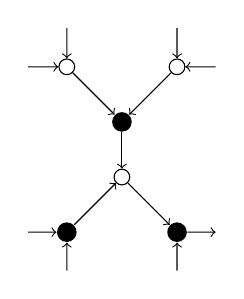
\begin{tikzpicture}[scale=.7]
 \node[circle,draw,inner sep=2pt](a)at(-1,1.5){};
 \node[circle,draw,inner sep=2pt](b)at(1,1.5){};
 \node[circle,fill=black,inner sep=2.5pt](c)at(0,.5){};
 \node[circle,draw,inner sep=2pt](d)at(0,-.5){};
 \node[circle,fill=black,inner sep=2.5pt](e)at(-1,-1.5){};
 \node[circle,fill=black,inner sep=2.5pt](f)at(1,-1.5){};
 \draw[->](a)--(c);\draw[->](b)--(c);\draw[->](c)--(d);
 \draw[->](e)--(d);\draw[->](d)--(f);
 \draw[->](-1,2.2)--(a);\draw[->](-1.7,1.5)--(a);
 \draw[->](1,2.2)--(b);\draw[->](1.7,1.5)--(b);
 \draw[->](-1,-2.2)--(e);\draw[->](-1.7,-1.5)--(e);
 \draw[->](1,-2.2)--(f);\draw[->](f)--(1.7,-1.5);
\end{tikzpicture}
\end{center}
$\mathcal T$ 上任意一条顺流而下的无限流
$\circ\longrightarrow\bullet\longrightarrow\circ\longrightarrow\bullet\longrightarrow\cdots$
唯一确定一条河流。显然，两条这样的流确定同一条河流，当且仅当它们在下游某处相遇。

\paragraph*{3.6.}
设 $\xi\in\operatorname{Pl}(L/k)$。由于 $\xi_{is}$（$i=1,2$）在 $\F_q$ 上互相共轭，$\xi_{1s}$ 为普通点当且仅当 $\xi_{2s}$ 为普通点；此时称 $\xi$ 普通。每个普通 $\xi$ 如下确定 $\mathcal T$ 上的河流 $\operatorname{Riv}(\xi)$。设 $A=V_1g_1$、$B=V_2g_2$ 相邻，取 $g\in V_1g_1\cap V_2g_2$。令 $\zeta$ 为 $g\xi$ 限制到 $K_0$ 后作为 $\overline X_{0\eta}$ 的点，$\zeta_s$ 为其在 $\overline X_{0s}$ 上的唯一特化。因为 $\xi$ 普通，$g\xi$ 也普通，所以 $\zeta_s$ 不属于 $\Pi\cap{}^t\Pi$（在 $\overline X_{0s}$ 上取交），而恰属于 $\Pi,{}^t\Pi$ 之一。若属于 $\Pi$，赋方向 $A\longrightarrow B$；若属于 ${}^t\Pi$，则取反向。容易看出，这在 $\mathcal T$ 上定义了河流 $\rho=\operatorname{Riv}(\xi)$。

取该河流的任意无限流 $[A_0\longrightarrow A_1\longrightarrow\cdots]$，及 $g\in D_\xi^+$（$\mathcal X$ 对称时，分别取 $g\in D_\xi$）。$g$ 保持 $\operatorname{Riv}(\xi)$，因此原流在 $g$ 下的像 $[A_0^g\longrightarrow A_1^g\longrightarrow\cdots]$ 为同河流的另一条流。两者必在下游某处相遇，所以当 $i$ 足够大时，对某个 $\delta\in\Z$ 有 $A_i^g=A_{i+\delta}$，且 $\delta$ 与原流的选取无关。映射 $g\mapsto\delta(g)$ 定义同态 $\delta:D_\xi^+\longrightarrow\Z$（分别地，$D_\xi\longrightarrow\Z$），容易看出
\[
 \operatorname{Deg}(g)=|\delta(g)|,\qquad g\in D_\xi^+
 \text{（分别地，}D_\xi\text{）}.\tag{3.6.1}
\]
特别地，$I_\xi^0$ 为 $\delta|_{I_\xi^+}$（分别地，$\delta|_{I_\xi}$，因为 $I_\xi^0\subset I_\xi^+$）的核；故只要 $\xi$ 普通，$I_\xi^0$ 总为 $I_\xi^+$（分别地，$I_\xi$）的正规子群，且 $I_\xi^+/I_\xi^0\simeq0$ 或 $\Z$（分别地，$I_\xi/I_\xi^0\simeq0$ 或 $\Z$）。

\paragraph*{3.7. 映射 $\chi$.}
令 $i=1,2$。若 $\overline X_{i\eta}$ 的点 $\xi_i$ 在 $\overline X$ 上的特化普通，则称 $\xi_i$ 普通。记全体普通点的集合为 $(\overline X_{i\eta})^{\mathrm{ord}}$。如下定义
$(\overline X_{1\eta})^{\mathrm{ord}}\sqcup(\overline X_{2\eta})^{\mathrm{ord}}$ 到自身的映射 $\chi$。给定 $\xi_1\in(\overline X_{1\eta})^{\mathrm{ord}}$（分别地，$\xi_2\in(\overline X_{2\eta})^{\mathrm{ord}}$），令 $\zeta$（分别地，$\zeta'$）为 $\overline X_{0\eta}$ 上满足 $\overline\varphi_1(\zeta)=\xi_1$（分别地，$\overline\varphi_2(\zeta')=\xi_2$）、且在 $\overline X_{0s}$ 上的特化位于 $\Pi$（分别地，${}^t\Pi$）的唯一点，其中 $\overline\varphi_i=\varphi_i\otimes_k\overline k$。定义
\[
 \chi(\xi_1)=\overline\varphi_2(\zeta),\qquad
 \chi(\xi_2)=\overline\varphi_1(\zeta').
\]
因此 $\chi$ 将两种普通点集合互相映入。一般而言，$\chi$ 是一个 $q$ 对一的映射。在 Kronecker CR 系统情形，Tate、Deligne、Dwork 已研究 $\chi$ 的一个重要 $p$ 进解析性质，即刚性（见[3]）。

\paragraph*{3.8. $\chi$ 的图示.}
取任意普通的 $\xi\in\operatorname{Pl}(L/k)$，令
\[
 (G_{\mathfrak p}^+\xi)_i=\{(g\xi)_i:g\in G_{\mathfrak p}^+\},
 \qquad i=1,2.\tag{3.8.1}
\]
不交并 $(G_{\mathfrak p}^+\xi)_1\sqcup(G_{\mathfrak p}^+\xi)_2$ 为 $\overline X_{1\eta}\sqcup\overline X_{2\eta}$ 的点集的子集，可自然识别为
\[
 (V_1\backslash G_{\mathfrak p}^+/I_\xi^+)
 \sqcup(V_2\backslash G_{\mathfrak p}^+/I_\xi^+)
 =\mathcal T^0/I_\xi^+.\tag{3.8.2}
\]
此外，$\chi$ 的作用对应于 $\operatorname{Riv}(\xi)$ 在 $\mathcal T$ 上确定的箭头，即
\[
 \{(G_{\mathfrak p}^+\xi)_1\sqcup(G_{\mathfrak p}^+\xi)_2
 \text{ 及 }\chi\text{ 的作用}\}
 =\{\mathcal T\text{ 及 }\operatorname{Riv}(\xi)\}/I_\xi^+.
\]
例如，当 $I_\xi^0=\{1\}$、$I_\xi^+\simeq\Z$、$q=2$ 时，此商如下：
\begin{center}
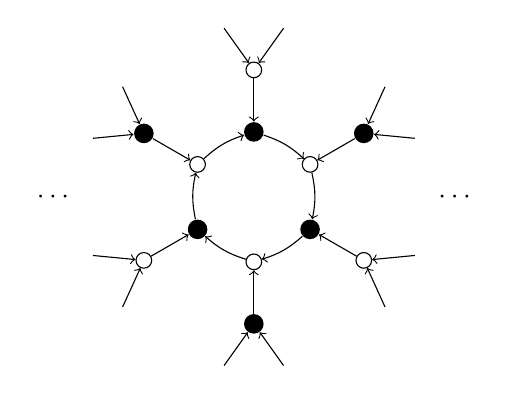
\begin{tikzpicture}[scale=.75]
 \foreach \j in {0,...,5}{
  \pgfmathtruncatemacro{\nx}{mod(\j+1,6)}
  \ifodd\j
   \node[circle,draw,fill=white,inner sep=2pt](n\j)at({90-60*\j}:1.1){};
   \node[circle,fill=black,inner sep=2.5pt](b\j)at({90-60*\j}:2.15){};
  \else
   \node[circle,fill=black,inner sep=2.5pt](n\j)at({90-60*\j}:1.1){};
   \node[circle,draw,fill=white,inner sep=2pt](b\j)at({90-60*\j}:2.15){};
  \fi
  \draw[->](b\j)--(n\j);
  \draw[->]({80-60*\j}:2.9)--(b\j);
  \draw[->]({100-60*\j}:2.9)--(b\j);
 }
 \foreach \j in {0,...,5}{\pgfmathtruncatemacro{\nx}{mod(\j+1,6)}\draw[->](n\j)to[bend left=12](n\nx);}
 \node at (-3.4,0){$\cdots$};\node at (3.4,0){$\cdots$};
\end{tikzpicture}\qquad(3.8.3)
\end{center}
中心圈的长度等于 $\operatorname{Deg}^+(\xi)$。

\paragraph*{3.9. 概形 $T_{ij}(\mathfrak p^l)$.}
对每个满足
\[
 i-j\equiv l\pmod2,\qquad1\leq i,j\leq2,\quad l\geq0\tag{3.9.1}
\]
的 $i,j,l$，如下定义 $X_i\otimes_oX_j$ 的闭子概形 $T_{ij}(\mathfrak p^l)$。设 $A_1,A_2$ 为 $\mathcal T^0$ 中分别对应于 $V_1,V_2$ 的点。固定这样的 $i,j,l$，取 $\mathcal T^0$ 中满足 $l(A_i,B)=l$ 的任意点 $B$。则 $l(A_j,B)$ 为偶数，所以对某个 $g\in G_{\mathfrak p}^+$，有 $B=A_j^g$。双陪集 $V_jgV_i$ 与 $B$ 的选取无关。考虑环同态
\[
 K_i\otimes_kK_j\longrightarrow K_iK_j^g\subset L,
 \qquad\sum_\lambda u_\lambda\otimes v_\lambda
 \longmapsto\sum_\lambda u_\lambda v_\lambda^g.
\]
其核定义 $X_i\times_oX_j$ 的一个闭整子概形，只依赖于 $i,j,l$，称为 $T_{ij}(\mathfrak p^l)$。容易证明 $T_{ji}(\mathfrak p^l)={}^tT_{ij}(\mathfrak p^l)$。当 $\mathcal X$ 对称时，它为对称的，且只依赖于 $l$。

\begin{originaltheorem}{命题 3.9.2（Proposition 3.9.2）}
设 $T_{ij}(\mathfrak p^l)_s$ 为 $T_{ij}(\mathfrak p^l)$ 的特殊纤维。则它是 $X\times_{\F_q}X$ 的闭子概形，由以下两性质确定：(i) 局部由单个方程定义；(ii) 不可约分支及其重数由下式给出：
\begin{align*}
 T_{ij}(\mathfrak p^l)_s
 &=(\Pi^l+{}^t\Pi^l)
 +\sum_{1\leq h<l/2}q^{h-1}(q-1)(\Pi^{l-2h}+{}^t\Pi^{l-2h})\\
 &\quad+\epsilon(l)q^{(l-2)/2}(q-1)\Delta,
\end{align*}
其中 $\Pi^r$ 为 $X$ 的 $q^r$ 次幂态射的图，${}^t\Pi^r$ 为其转置图，$\Delta$ 为 $X\times_{\F_q}X$ 的对角线；当 $l$ 为偶数时 $\epsilon(l)=1$，为奇数时 $\epsilon(l)=0$。\footnote{\textbf{译者注（本次校订）：}本公式适用于 $l\ge1$。前文的定义也允许 $l=0$，但此时应单独取 $T_{ii}(\mathfrak p^0)_s=\Delta$；直接代入所列公式会得到错误的对角线重数。}
\end{originaltheorem}

\paragraph*{3.10. 典范提升.}
令 $i=1$ 或2，$l\geq1$。对 $\overline X$ 上在 $\F_{q^2}$ 上次数为 $l$ 的每个普通点 $x$，将定义其典范提升 $\xi_i\in\overline X_{i\eta}$。由 $i-j\equiv l\pmod2$ 定义 $j=1$ 或2，考虑命题3.9.2。注意，$\overline X$ 中在 $\F_{q^2}$ 上次数为 $l$ 的点，与 $\Pi^l\cap{}^t\Pi^l$ 中不属于 $T_{ij}(\mathfrak p^l)_s$ 的任何其他不可约分支的几何点，通过 $x\leftrightarrow(x,x^{q^l})$ 一一对应。

\begin{originaltheorem}{命题 3.10.1（Proposition 3.10.1）}
若 $x$ 普通，则 $(x,x^{q^l})$ 不是二维概形 $T_{ij}(\mathfrak p^l)$ 的正规点。
\end{originaltheorem}
取 $T_{ij}(\mathfrak p^l)$ 的正规化到 $X_0$ 的适当态射，即可证明此命题。下述引理是典范提升的关键，它是二维局部环的一个初等练习。

\begin{originaltheorem}{引理 3.10.2（Lemma 3.10.2）}
设 $R$ 为任意完备离散赋值环，$k$、$\kappa$ 分别为其分式域和剩余域，$\Spec R=\{\eta,s\}$（$s$ 为闭点）。设 $Z$ 为具有固有平坦 $R$ 概形结构的二维整概形，$z$ 为 $Z_s=Z\otimes_R\kappa$ 的一个 $\kappa$ 有理普通二重点（ordinary double point），且 $z$ 在 $Z$ 上非正规。则 $Z_\eta$ 上有唯一非正规点 $\zeta$，其特化为 $z$；而且 $\zeta$ 为 $Z_\eta$ 的 $k$ 有理普通二重点。
\end{originaltheorem}
由于 $z$ 在 $Z_s$ 上约化（因为它是普通二重点），且 $Z$ 在 $R$ 上平坦，二维局部环 $\mathcal O_{Z,z}$ 为 Cohen--Macaulay 环（Cohen--Macaulay ring）。由 Serre 正规性判别法（Serre's criterion for normality）[4, IV, 5.8.6]，得到 $\zeta$ 的存在性。唯一性及最后断言来自完备化的同构\footnote{\textbf{译者注（本次校订）：}下列完成局部环的表达式要求普通二重点是分裂的，即两条切线都定义在剩余域 $\kappa$ 上；一般的普通二重点需先作适当的非分歧扩张。在下文的应用中，两条分支来自 $\Pi^l$ 与 ${}^t\Pi^l$，已在所取剩余域上定义，故满足这一条件。}
\[
 \widehat{\mathcal O}_{Z,z}\simeq R[[X,Y]]/(XY).
\]

将引理3.10.2用于 $R=o_{2l}$、$Z=T_{ij}(\mathfrak p^l)\otimes_oo_{2l}$、$z=(x,x^{q^l})$，得到：
\begin{originaltheorem}{定理 3.10.3（Theorem 3.10.3）}
设 $i,j,l,x$ 如§3.10开头。则 $T_{ij}(\mathfrak p^l)_\eta$ 上存在唯一的非正规 $k_{2l}$ 有理点 $(\xi_i,\xi'_j)$，其中 $\xi_i\in\overline X_{i\eta}$、$\xi'_j\in\overline X_{j\eta}$，它提升 $(x,x^{q^l})$。此外，$(\xi_i,\xi'_j)$ 是 $T_{ij}(\mathfrak p^l)_\eta\otimes_kk_{2l}$ 的普通二重点。
\end{originaltheorem}
\begin{originaltheorem}{定义 3.10.4（Definition 3.10.4）}
$\xi_i$ 为 $x$ 在 $\overline X_{i\eta}$ 上的典范提升。
\end{originaltheorem}

\paragraph*{3.11.}
由 $(\xi_i,\xi'_j)$ 的唯一性，可以推出典范提升的以下基本性质。首先，因为 $T_{ji}(\mathfrak p^l)={}^tT_{ij}(\mathfrak p^l)$，定义和唯一性立即表明，$\xi'_j$ 是 $x^{q^l}$ 在 $\overline X_{j\eta}$ 上的典范提升。此外，还有以下重要性质：
\begin{originaltheorem}{定理 3.11.1（Theorem 3.11.1）}
设 $x$ 为 $\overline X$ 的普通点，$\xi_i$ 为 $x$ 在 $\overline X_{i\eta}$ 上的典范提升（$i=1,2$），令 $d=\operatorname{Deg}(x/\F_q)$。则：

(i) $\xi_i$ 为 $k_d$ 有理点，且在 $k$ 上的次数为 $d$；

(ii) $\xi_i^{[q]}$ 是 $x^q$ 在 $\overline X_{i\eta}$ 上的典范提升；

(iii) $\chi(\xi_1)$（分别地，$\chi(\xi_2)$）是 $x^q$ 在 $\overline X_{2\eta}$（分别地，$\overline X_{1\eta}$）上的典范提升；

(iv) $\xi_i$ 是 $\overline X_{i\eta}$ 上唯一特化为 $x$、且满足 $\chi^{2d}(\xi_i)=\xi_i$ 的点；

(v) 当 $\mathcal X$ 对称时，$\xi_1=\xi_2$。
\end{originaltheorem}

对于 Kronecker CR 系统，典范提升就是 Deuring 提升：将 $\overline\F_p$ 上一条非超奇异椭圆曲线的 $j$ 不变量，提升到 $\overline\Q_p$ 上一条具有相同自同态环（endomorphism ring）的椭圆曲线的 $j$ 不变量。刻画(iv)沿用了 Dwork [3] 对 Deuring 提升的刻画。

\paragraph*{3.12.}
固定 $i$，考虑将 $\overline X$ 的普通点提升到 $\overline X_{i\eta}$ 的典范提升 $x\mapsto\xi_i$。由定理3.11.1，它将 $X\otimes_{\F_q}\F_{q^2}$ 的每个普通闭点
$(x,x^{q^2},\ldots,x^{q^{2l-2}})$（$l=\operatorname{Deg}(x/\F_{q^2})$）提升为 $X_{i\eta}\otimes_kk_2$ 的闭点
$(\xi_i,\xi_i^{[q]^2},\ldots,\xi_i^{[q]^{2l-2}})$。又因为 $\xi_i^{[q]^2}=\chi^2(\xi_i)$，各 $\xi_i,\xi_i^{[q]^2},\ldots$ 到 $\operatorname{Pl}(L/k)$ 的延拓属于同一 $G_{\mathfrak p}^+$ 轨道 $G_{\mathfrak p}^+\xi$。因为 $\chi^{2l}(\xi_i)=\xi_i$，$I_\xi^+$ 包含满足 $\delta(g)=2l$ 的元素 $g$。由此容易证明，$G_{\mathfrak p}^+\xi$ 属于 $\operatorname{Pl}(L/k;[A])$ 的轨道，$\operatorname{Deg}^+(\xi)=2l$，且 $D_\xi^+/I_\xi^+$ 诱导 $\mathcal O_\xi/\mathfrak m_\xi$ 在 $k_2\cap(\mathcal O_\xi/\mathfrak m_\xi)$ 上的完整自同构群。因此，定理3.4.1只剩最后一步：证明“这些 $G_{\mathfrak p}^+\xi$ 穷尽了 $G_{\mathfrak p}^+\backslash\operatorname{Pl}(L/k;[A])$”。

证明如下。先用命题3.9.2计算 $X_{i\eta}\times_kX_{i\eta}$ 上交积（intersection product）$T_{ii}(\mathfrak p^{2l})_\eta\cdot\Delta_\eta$ 的次数。再利用 $\operatorname{Riv}(\xi)$，计数该交积中满足下述条件的不同点：或属于典范提升在 $G_{\mathfrak p}^+$ 下的变换，或不对应于 $\operatorname{Pl}(L/k;[A])$ 中的元素。可以验证，所数得的不同点数恰好等于交积的次数，从而得到所需的穷尽性。细节[9b]即将发表。

\paragraph*{3.13.}
由定理3.11.1还可得进一步结论。例如，对每个 $\xi\in\operatorname{Pl}(L/k;[A])$，剩余域 $\mathcal O_\xi/\mathfrak m_\xi$ 在 $(\mathcal O_\xi/\mathfrak m_\xi)\cap k_2$ 上阿贝尔；当 $\mathcal X$ 对称时，在 $k$ 上也阿贝尔，而且其范数群（norm group）可显式确定。忽略分歧的影响，可以粗略地说，这个范数群由 $T_{ii}(\mathfrak p^{2l})_\eta$ 在 $(\xi_i,\xi_i)$ 处的斜率确定。在这一步使用 Lubin--Tate 的工作[12]。

\paragraph*{3.14. 第一个主定理（The First Main Theorem）.}
现在设 $\mathcal X$ 为关于 $(X,o)$ 的非分歧对称 CR 系统。固定嵌入 $\epsilon:k\hookrightarrow\C$，令 $\Gamma$ 为属于 $\mathcal X,\epsilon$ 的算术基本群（§2.9）。§§3.14--3.15将用 $\Gamma$ 重新表述定理3.4.1与3.11.1。

如§2.9，取 $\Sigma$ 的连通分支 $\Sigma_0$，将其与 $\mathfrak H$ 等同，并把 $\Gamma=\{\gamma\in G_{\mathfrak p}:\gamma\Sigma_0=\Sigma_0\}$ 看作 $\mathfrak H$ 的变换群。对每个 $\tau\in\mathfrak H$，记其在 $\Gamma$ 中的稳定子群为 $\Gamma_\tau$，令
\[
 \mathcal H=\{\tau\in\mathfrak H:|\Gamma_\tau|=\infty\}.\tag{3.14.1}
\]
显然 $\mathcal H$ 是 $\mathfrak H$ 的 $\Gamma$ 稳定子集。称其点为 $\mathfrak H$ 上的 $\Gamma$ 点（$\Gamma$-point）。

\begin{originaltheorem}{主定理 I（Main Theorem I）}
记 $X$ 的全部普通闭点集合为 $\mathfrak P(X)$。则模 $\mathfrak p$ 约化诱导双射
\[
 i_\Gamma:\Gamma\backslash\mathcal H\xrightarrow{\sim}\mathfrak P(X).\tag{3.14.2}
\]
\end{originaltheorem}
这是定理3.4.1(ii)的直接推论，因为 $\Gamma\backslash\mathcal H$ 与 $G_{\mathfrak p}\backslash\operatorname{Pl}(L/k;[A])$ 之间存在如下典范双射。首先，若 $\Sigma$ 的元素在 $G_{\mathfrak p}$ 中有非平凡稳定子群，则它在 $k$ 上代数，所以 $\mathcal H$ 嵌入 $\operatorname{Pl}(L/k)$。此外，对任意 $\tau\in\mathfrak H\cap\operatorname{Pl}(L/k)$，$\Gamma_\tau$ 正是§3.2的惯性群 $I_\tau$。因为在非分歧情形条件[A]等价于 $|I_\tau|=\infty$（§3.3），故
$\mathfrak H\cap\operatorname{Pl}(L/k;[A])=\mathcal H$。$G_{\mathfrak p}$ 在 $\Sigma$ 的全部连通分支上可迁，从而诱导上述双射。

\paragraph*{3.15.}
主定理I给出了简洁的表述。关于几何点的约化与提升，还有更精细的信息，下面用 $\Gamma$ 加以描述。设 $\Delta_i$（$i=1,2$）为对应于 $V_i$ 的 $\Gamma$ 子群（§2.9）。则 $\Delta_i\backslash\mathfrak H$ 可与 $X_{i\C}=X_{i\eta}\otimes_{k_c}\C$ 的点集等同，其中张量积使用由 $\Sigma_0$ 限制到 $k_c$ 定义的嵌入 $k_c\hookrightarrow\C$。设 $x$ 为 $X$ 上在 $\F_q$ 上次数为 $d$ 的几何点，$P=(x,x^q,\ldots,x^{q^{d-1}})$ 为包含 $x$ 的闭点。记 $\mathcal H^P$ 为满足下述条件的全体 $\tau\in\mathcal H$：含 $\tau$ 的 $\Gamma$ 轨道经 $i_\Gamma$ 对应于 $P$。

\emph{情形1。} 此时 $\Gamma$ 包含满足(2.9.5)的对合 $\iota$，所以 $i$ 的两种选取没有区别。商 $\Delta_1\backslash\mathcal H^P\subset X_{1\C}$ 如图：
\begin{center}
\begin{tikzpicture}[scale=.8]
 \foreach \j in {0,...,3}{
  \node[circle,draw,inner sep=2pt](c\j)at({90-90*\j}:.8){};
  \node[circle,draw,inner sep=2pt](b\j)at({90-90*\j}:1.8){};
  \draw[->](b\j)--(c\j);
  \draw[->]({80-90*\j}:2.4)--(b\j);
  \draw[->]({100-90*\j}:2.4)--(b\j);
 }
 \foreach \j in {0,...,3}{\pgfmathtruncatemacro{\nx}{mod(\j+1,4)}\draw[->](c\j)to[bend left=18](c\nx);}
 \node[anchor=west]at(2.7,0){$q=2,\ d=4$};
\end{tikzpicture}\qquad(3.15.1)
\end{center}
箭头为 $q$ 对一的 $\chi$ 映射，中心圈长度为 $d$，由 $x^{q^\nu}$（$0\leq\nu<d$）在 $\overline X_1$ 上的典范提升组成。

\emph{情形2。} $\mathcal X$ 上的共同 $o_2$ 结构使 $X_1$ 与 $X_2$ 的结构互为共轭。因此 $X_{1\C},X_{2\C}$ 一般不同构。不交并 $(\Delta_1\backslash\mathcal H^P)\sqcup(\Delta_2\backslash\mathcal H^P)$ 如图(3.8.3)，其中空心点属于前者，实心点属于后者，箭头为 $\chi$ 映射，中心圈长度为 $d$（为偶数），由 $x^{q^\nu}$ 在 $\overline X_{i\C}$ 上的典范提升组成，$i$ 由 $\nu$ 的奇偶性区分。

最后，两种情形中 $\Gamma_\tau$ 均为无限循环群，且§3.6的同态 $\delta:D_\tau\longrightarrow\Z$ 诱导同构 $\Gamma_\tau\simeq d\Z$。所以若 $\gamma_\tau$ 是 $\Gamma_\tau$ 的生成元，则 $P$ 在 $\F_q$ 上的次数 $d$ 等于 $\operatorname{Deg}(\gamma_\tau)$，这里将 $\gamma_\tau$ 视为 $G_{\mathfrak p}$ 的元素。还可以用 $\delta(\gamma_\tau)$ 的正负区分两个生成元。这个符号也有如下解释：设 $\gamma_\tau$ 在 $\tau$ 处的切空间上诱导线性变换 $d/dz\mapsto\lambda\,d/dz$。则通过嵌入 $\epsilon:k\longrightarrow\C$，有 $\lambda\in k^\times$，且 $\operatorname{ord}_{\mathfrak p}\lambda$ 与 $\delta(\gamma_\tau)$ 同号。

\origsection{4}{第二 Galois 理论（The second Galois theory）}
第二 Galois 理论研究以相容方式连接两个 CR 系统 $\mathcal X$ 与 $\mathcal X^*$ 的三个有限平展态射（finite étale morphism）$f_i:X_i^*\longrightarrow X_i$ 所组成的系统 $\widehat f=(f_1,f_0,f_2)$。§4给出由 $\widehat f\mapsto\widehat f\otimes\C$ 与 $\widehat f\mapsto\widehat f\otimes\F_q$ 诱导的两个范畴等价的主要结果。其中前一个等价尤其深刻。

\paragraph*{4.1.}
一般地，设 $\mathcal U=\{U_1\xleftarrow{\phi_1}U_0\xrightarrow{\phi_2}U_2\}$ 为三个概形和两个态射组成的系统，$\mathcal U^*=\{U_1^*\xleftarrow{\phi_1^*}U_0^*\xrightarrow{\phi_2^*}U_2^*\}$ 为另一同类系统。若 $\widehat f$ 为三个有限平展态射 $f_i:U_i^*\longrightarrow U_i$ 所成的三元组，满足 $f_i\circ\phi_i^*=\phi_i\circ f_0$，且典范地 $U_0^*\simeq U_i^*\times_{U_i}U_0$（$i=1,2$），则称 $(\mathcal U^*,\widehat f)$ 为 $\mathcal U$ 的有限平展覆盖（finite étale covering）。

现在设 $\mathcal X$、$\mathcal X^*$ 分别为关于 $(X,o)$、$(X^*,o)$ 的 CR 系统，基环 $o$ 相同。假设 $(\mathcal X^*,\widehat f)$ 为 $\mathcal X$ 的有限平展覆盖，且 $f_i$ 都为 $o$ 态射，则称其为有限平展 CR 覆盖（finite étale CR-covering）。由定义，通过基变换（base change）$\otimes_o\F_q$ 从 $f_1,f_2$ 得到的两个有限平展态射 $f_{is}:X^*\longrightarrow X$ 必须相同，记为 $f$。容易得到 $\mathfrak S^*=f^{-1}(\mathfrak S)$，其中两者分别为 $\mathcal X^*,\mathcal X$ 的特殊点集合。若 $\mathcal X$ 非分歧，则 $\mathcal X^*$ 也非分歧，因为 $\varphi_{i\eta}^*$ 是 $\varphi_{i\eta}$ 的基变换。若 $\mathcal X$ 对称，则利用[4, IV, 18.3.4]容易证明 $\mathcal X^*$ 也对称。

\paragraph*{4.2.}
设 $\mathcal X$ 为任意非分歧对称 CR 系统，固定嵌入 $\epsilon:k\hookrightarrow\C$，令 $\Gamma$ 为其算术基本群。第二 Galois 理论的主要结果如下。
\begin{originaltheorem}{主定理 II（Main Theorem II）}
下列三个范畴典范等价：

(i) $\mathcal X$ 的有限平展 CR 覆盖 $(\mathcal X^*,\widehat f)$；

(ii) $\Gamma$ 的有限指数子群 $\Gamma^*$；

(iii) 有限平展覆盖 $f:X^*\longrightarrow X$，其中 $X^*$ 连通，且位于 $X$ 的特殊点 $x_1,\ldots,x_H$ 上方的全部点均为 $X^*$ 的 $\F_{q^2}$ 有理点。
\end{originaltheorem}
等价函子如下：(i)$\longrightarrow$(ii) 为取算术基本群；(i)$\longrightarrow$(iii) 为§4.1所述函子。这里省略证明。(i)$\sim$(iii)的证明与[6]相同；(i)$\sim$(ii)的证明更为精细，其关键是曲线的非分歧覆盖具有良约化（good reduction）的判别法[8]；我们用 Frobenius 的适当提升建立了这一判别法。

\origsection{5}{同时单值化与互反律（Simultaneous uniformizations and reciprocity）}
在§5中，$\mathcal X$ 为关于 $(X,o)$ 的非分歧对称 CR 系统，$\epsilon:k\hookrightarrow\C$ 固定，$\Gamma$ 为其算术基本群。

\paragraph*{5.1.}
设 $\Gamma^*\subset\Gamma$ 为有限指数子群，$(\mathcal X^*,\widehat f)$ 为相应有限平展 CR 覆盖，$(X^*,f)$ 为相应的 $X$ 的有限平展覆盖（§4）。用 $\mathcal H$（分别地 $\mathcal H^*$）表示 $\mathfrak H$ 上的全部 $\Gamma$ 点（分别地 $\Gamma^*$ 点），见§3.14。由于对每个 $\tau\in\mathfrak H$ 均有 $(\Gamma_\tau:\Gamma_\tau^*)<\infty$，故 $\mathcal H^*=\mathcal H$。用 $\mathfrak P(X^*)$ 表示关于 $\mathcal X^*$ 的全部普通闭点。如§4所述，$\mathfrak P(X^*)=f^{-1}(\mathfrak P(X))$。由 $\mathcal X^*$ 的主定理I，模 $\mathfrak p$ 约化给出典范双射
\[
 i_{\Gamma^*}:\Gamma^*\backslash\mathcal H\xrightarrow{\sim}\mathfrak P(X^*).\tag{5.1.1}
\]
若 $X^*/X$ 为 Galois 覆盖，$P^*$ 为 $X^*$ 的闭点，则按定义，Frobenius 自同构 $((X^*/X)/P^*)$ 为 $\Gal(X^*/X)$ 中在 $P^*$ 的几何点上以 $q^d$ 次幂映射作用的元素 $\sigma$，其中 $d$ 为 $P^*$ 下方 $X$ 的闭点 $P$ 在 $\F_q$ 上的次数。由于 Galois 群元素在点上从左作用，在函数上从右作用，且通过 $f^\sigma(\xi)=f(\sigma\xi)$ 联系，几何与算术 Frobenius 在这里不写为互逆表达式。

\begin{originaltheorem}{主定理 III（Main Theorem III）}
(i) 下图交换：
\[
\begin{tikzcd}[column sep=large,row sep=large]
 \Gamma^*\backslash\mathcal H \arrow[r,"i_{\Gamma^*}"] \arrow[d,"\text{典范映射}"'] &
 \mathfrak P(X^*) \arrow[d,"f"]\\
 \Gamma\backslash\mathcal H \arrow[r,"i_\Gamma"'] & \mathfrak P(X).
\end{tikzcd}\tag{5.1.2}
\]

(ii) 若 $\Gamma^*$ 在 $\Gamma$ 中正规，则 $\Gamma/\Gamma^*$ 在 $\Gamma^*\backslash\mathcal H$ 上的自然作用，与 $\Gal(X^*/X)$ 在 $\mathfrak P(X^*)$ 上的作用，经 $i_{\Gamma^*}$ 及主定理II的典范同构 $\Gamma/\Gamma^*\simeq\Gal(X^*/X)$ 相互对应。

(iii) 此外，$\Gamma^*$ 正规时，$P_\tau^*=i_{\Gamma^*}(\Gamma^*\tau)$（$\tau\in\mathcal H$）在 $X$ 上的 Frobenius 自同构由 $\Gamma^*\gamma_\tau$ 给出，其中 $\gamma_\tau$ 为 $\Gamma_\tau$ 中满足 $\delta(\gamma_\tau)<0$ 的生成元（§3.15），即
\[
 \left(\frac{X^*/X}{P_\tau^*}\right)=\Gamma^*\gamma_\tau.\tag{5.1.3}
\]
\end{originaltheorem}
因此，Frobenius 自同构的这一统一描述可简记为
\[
 \left(\frac{/X}{\tau}\right)=\gamma_\tau.\tag{5.1.4}
\]

\origsection{6}{Shimura 曲线的情形（The case of Shimura curves）}
由定理6.3.3，即 Shimura 同余关系的“$\mathfrak p$ 典范版本”，上述结果对每条 Shimura 曲线的几乎所有 $\mathfrak p$ 适用。

\paragraph*{6.1.}
设 $F$ 为次数 $m$ 的全实代数数域，$B$ 为 $F$ 上四元数代数（quaternion algebra），在一个无穷素点 $\infty_1$ 处非分歧，在其余全部无穷素点 $\infty_2,\ldots,\infty_m$ 处分歧。照例，下标 $\mathfrak l,\A,R$ 分别表示局部化、阿代尔化及阿代尔的无穷部分。$B/F$ 及其局部化等的约化范数（reduced norm）记为 $N(*)$。对任意 $b_R\in B_R^\times$，$N(b_R)$ 在 $\infty_2,\ldots,\infty_m$ 处为正。用 $(B_\A^\times)^+$ 表示满足 $N(b_R)$ 全正（totally positive）的全部 $b_\A$ 组成的群，令 $(B_R^\times)^+=(B_\A^\times)^+\cap B_R^\times$。

设 $\mathfrak L$ 为 Shimura [15] 对 $B/F$ 构造的 $F$ 上函数域，取其中“$n=r=1$”的情形。它是 $F$ 的无限生成一维扩张，由 $B$ 上算术自守函数的全域得到。Shimura 在[15]建立同构
\[
 \Aut(\mathfrak L/F)\simeq
 (B_\A^\times)^+/\overline{(B_R^\times)^+F^\times},\tag{6.1.1}
\]
其中横线表示拓扑闭包。回忆，$F$ 在 $\mathfrak L$ 中的代数闭包为 $F$ 的最大阿贝尔扩张 $F^{\mathrm{ab}}$，且下图交换：
\[
\begin{tikzcd}[column sep=large,row sep=large]
 (B_\A^\times)^+ \arrow[r,"t"] \arrow[d,"N^{-1}"'] &
 \Aut(\mathfrak L/F) \arrow[d,"\rho"]\\
 F_\A^\times \arrow[r,"c"'] & \Aut(F^{\mathrm{ab}}/F).
\end{tikzcd}\tag{6.1.2}
\]
这里 $t$ 由(6.1.1)定义，$c$ 为类域论（class field theory）定义的同态，$\rho$ 为限制同态，$N^{-1}(b_\A)=N(b_\A)^{-1}$。

对 $\Aut(\mathfrak L/F)$ 的每个紧开子群 $\mathcal U$，记其在 $\mathfrak L$（分别地，$F^{\mathrm{ab}}$）中的不动域为 $\mathfrak L^{\mathcal U}$（分别地，$(F^{\mathrm{ab}})^{\mathcal U}$）。则 $\mathfrak L^{\mathcal U}$ 为 $(F^{\mathrm{ab}})^{\mathcal U}$ 上一元代数函数域。令 $S(\mathcal U)$ 为以 $\mathfrak L^{\mathcal U}$ 为函数域的固有光滑曲线，称其为对应于 $\mathcal U$ 的 Shimura 曲线。

\paragraph*{6.2.}
设 $\mathfrak p$ 为 $F$ 的一个有限素点，$B$ 在该处非分歧。将 $F_{\mathfrak p}^\times$ 视为 $(B_\A^\times)^+$ 的中心子群，令 $P$ 为 $t(F_{\mathfrak p}^\times)$ 的闭包。则 $P$ 为 $\Aut(\mathfrak L/F)$ 的中心紧子群。设 $k^{(1)}$、$k^{(\infty)}$ 分别为 $\mathfrak p$ 在 $F^{\mathrm{ab}}/F$ 中的分解域、惯性域，$k^{(d)}$（$d\geq1$）为 $k^{(\infty)}/k^{(1)}$ 的唯一 $d$ 次子扩张。令 $\mathfrak L^P$ 为 $P$ 的不动域，则 $\mathfrak L^P\cap k^{(\infty)}=k^{(2)}$。
令
\[
 B_\Lambda^\times=\prod'_{\mathfrak l\ne\infty,\mathfrak p}B_{\mathfrak l}^\times,
 \qquad F_\Lambda^\times=\prod'_{\mathfrak l\ne\infty,\mathfrak p}F_{\mathfrak l}^\times,\tag{6.2.1}
\]
其中 $\mathfrak l\ne\infty$ 简记 $\mathfrak l\ne\infty_1,\ldots,\infty_m$。对 $B_\A^\times$（分别地，$F_\A^\times$）的每个子群 $H$，用 $H^\sim$ 表示 $H$ 在 $B_\Lambda^\times$（分别地，$F_\Lambda^\times$）中投影的拓扑闭包。考虑典范同构
\begin{equation}
\begin{split}
 \Aut(\mathfrak L/F)/P
 &\simeq(B_\A^\times)^+/\overline{(B_R^\times)^+F_{\mathfrak p}^\times F^\times}\\
 &\simeq(B_{\mathfrak p}^\times/F_{\mathfrak p}^\times)
 \times(B_\Lambda^\times/(F^\times)^\sim).
\end{split}\tag{6.2.2}
\end{equation}
这些群自然作用于 $\mathfrak L^P$。令
\[
 B_\Lambda^{\times(1)}=
 \{b_\Lambda\in B_\Lambda^\times:N(b_\Lambda)\in((F^\times)^+)^\sim\},\tag{6.2.3}
\]
其中 $(F^\times)^+$ 为 $F$ 的全部全正元素构成的群。同构(6.2.2)诱导
\[
 \Aut(\mathfrak L/k^{(1)})/P
 \simeq(B_{\mathfrak p}^\times/F_{\mathfrak p}^\times)
 \times(B_\Lambda^{\times(1)}/(F^\times)^\sim).\tag{6.2.4}
\]

\begin{originaltheorem}{定义 6.2.5（Definition 6.2.5）}
对 $B_\Lambda^{\times(1)}/(F^\times)^\sim$ 的每个紧开子群 $U_\Lambda$，其在 $\mathfrak L^P$ 中的不动域，配以 $B_{\mathfrak p}^\times/F_{\mathfrak p}^\times$ 的自然作用，称为关联于 $U_\Lambda$ 的 $B_{\mathfrak p}^\times/F_{\mathfrak p}^\times$ 域，记为 $L=L(U_\Lambda)$。
\end{originaltheorem}
所以 $L(U_\Lambda)$ 为 $k^{(1)}$ 上的一维无限生成扩张，其上 $B_{\mathfrak p}^\times/F_{\mathfrak p}^\times$ 忠实作用。

\begin{originaltheorem}{定义 6.2.6（Definition 6.2.6）}
对每个 $U_\Lambda$，$\Gamma=\Gamma(U_\Lambda)$ 为 $B^\times/F^\times$ 中满足
\[
 \operatorname{pr}_{\infty_1}(\gamma)\in(B_{\infty_1}^\times)^+/\R^\times,
 \qquad\operatorname{pr}_\Lambda(\gamma)\in U_\Lambda
\]
的全部 $\gamma$ 所成子群。这里两投影分别从 $B^\times/F^\times$ 投到 $B_{\infty_1}^\times/\R^\times$ 与 $B_\Lambda^\times/(F^\times)^\sim$。
\end{originaltheorem}
由 Eichler--Kneser 逼近定理（Eichler--Kneser approximation theorem），$\Gamma(U_\Lambda)=\Gamma(U'_\Lambda)$ 蕴含 $U_\Lambda=U'_\Lambda$。

固定 $F_{\mathfrak p}$ 上同构 $B_{\mathfrak p}\simeq M_2(F_{\mathfrak p})$，诱导 $B_{\mathfrak p}^\times/F_{\mathfrak p}^\times\simeq\operatorname{PGL}_2(F_{\mathfrak p})$。设 $V_1,V_2$ 为分别对应于 $\operatorname{PGL}_2(o_{\mathfrak p})$、$w_{\mathfrak p}^{-1}\operatorname{PGL}_2(o_{\mathfrak p})w_{\mathfrak p}$ 的紧开子群，其中 $o_{\mathfrak p}$ 为整数环，
$w_{\mathfrak p}=\left(\begin{smallmatrix}0&1\\\pi&0\end{smallmatrix}\right)$，$\pi$ 为素元。令 $V_0=V_1\cap V_2$。给定 $U_\Lambda$，令 $L=L(U_\Lambda)$，$K_i$（$i=0,1,2$）为 $V_i$ 在 $L$ 中的不动域，即 $V_i\times U_\Lambda$ 在 $\mathfrak L^P$ 中的不动域。每个 $K_i$ 为 $k^{(1)}$ 上一元代数函数域，且 $K_0=K_1K_2$。此外，$w_{\mathfrak p}$ 诱导 $K_0$ 的对合 $\iota$，它在 $k^{(1)}$ 上平凡，并交换 $K_1,K_2$。$L$ 为使 $L/K_i$（$i=1,2$）均为 Galois 扩张的最小 $K_0$ 扩张。

设 $X_{i\eta}$ 为 $k^{(1)}$ 上以 $K_i$ 为函数域的固有光滑曲线，$\varphi_{i\eta}:X_{0\eta}\longrightarrow X_{i\eta}$ 为自然态射。则通过 $\iota$ 有 $X_{1\eta}=X_{2\eta}$，且 $X_{0\eta}$ 在 $X_{1\eta}\times_{k^{(1)}}X_{2\eta}$ 中的像 $T_\eta$ 满足 ${}^tT_\eta=T_\eta$。这样定义的系统
\[
 \{X_{1\eta}\xleftarrow{\varphi_{1\eta}}X_{0\eta}
 \xrightarrow{\varphi_{2\eta}}X_{2\eta}\}\tag{6.2.7}
\]
与同构 $B_{\mathfrak p}\simeq M_2(F_{\mathfrak p})$ 的选取无关。称其为关联于 $(\mathfrak p,U_\Lambda)$ 的 $k^{(1)}$ 系统。

$\mathfrak p$ 在 $k^{(1)}$ 中的每个延拓 $\widetilde{\mathfrak p}$ 定义 $k^{(1)}$ 到 $F_{\mathfrak p}$ 的 $\widetilde{\mathfrak p}$ 进嵌入。用 $\mathcal X(\widetilde{\mathfrak p},U_\Lambda)_\eta$ 表示通过此嵌入作基变换 $\otimes F_{\mathfrak p}$，由(6.2.7)得到的 $F_{\mathfrak p}$ 上曲线系统。

\begin{originaltheorem}{问题 6.2.8（Question 6.2.8）}
是否存在 $o_{\mathfrak p}$ 上的对称 CR 系统 $\mathcal X(\widetilde{\mathfrak p},U_\Lambda)$，以 $\mathcal X(\widetilde{\mathfrak p},U_\Lambda)_\eta$ 为一般纤维？
\end{originaltheorem}
Shimura 的工作在下述意义下对“几乎所有 $\mathfrak p$”给出了肯定答案，Y. Morita 又补充了若干“个别”$(\widetilde{\mathfrak p},U_\Lambda)$ 的结果。但据作者所知，这一问题的一般情形仍有待解决。注意，由主定理II（§4）及§4.1末句，若6.2.8对 $(\widetilde{\mathfrak p},U_\Lambda)$ 成立，且 $\varphi_{i\eta}$（$i=1,2$）非分歧，则它也对 $U_\Lambda$ 的每个开子群 $U_\Lambda^*$ 所对应的 $(\widetilde{\mathfrak p},U_\Lambda^*)$ 成立。

\paragraph*{6.3.}
设 $\mathfrak p$ 如§6.2。若 $\Aut(\mathfrak L/F)$ 的紧开子群 $\mathcal U$ 包含 $B_{\mathfrak p}^\times$ 的某个极大紧子群 $\widetilde V_{\mathfrak p}$ 的像 $t(\widetilde V_{\mathfrak p})$，则称 $\mathcal U$ 与 $\mathfrak p$ 互素。此时 $\widetilde V_{\mathfrak p}$ 唯一确定，称为 $\mathcal U$ 的 $\mathfrak p$ 分量。显然 $\mathcal U$ 与几乎所有 $\mathfrak p$ 互素。

设 $\mathcal U$ 与 $\mathfrak p$ 互素，则 $(F^{\mathrm{ab}})^{\mathcal U}\subset k^{(\infty)}$。令
\[
 \mathcal U^{(P)}=(\mathcal U\cap\Aut(\mathfrak L/k^{(\infty)}))P,\tag{6.3.1}
\]
$S(\mathcal U^{(P)})$ 为以 $\mathcal U^{(P)}$ 在 $\mathfrak L$ 中的不动域为函数域的固有光滑曲线。其全常数域为 $k^{(2)}$，且
\[
 S(\mathcal U^{(P)})\otimes k^{(\infty)}
 \simeq S(\mathcal U)\otimes k^{(\infty)},\tag{6.3.2}
\]
其中张量积在各自全常数域上取。由 $S(\mathcal U)\otimes k^{(\infty)}$ 模去 $P$ 作用得到的曲线 $S(\mathcal U^{(P)})$，称为 $S(\mathcal U)$ 的 $\mathfrak p$ 典范模型（$\mathfrak p$-canonical model）。把 $\mathcal U^{(P)}$ 视为群(6.2.4)的子群，它分解为 $V_{\mathfrak p}\times U_\Lambda$，其中 $V_{\mathfrak p}$ 为 $\widetilde V_{\mathfrak p}$ 在 $B_{\mathfrak p}^\times/F_{\mathfrak p}^\times$ 中的像，$U_\Lambda$ 为 $B_\Lambda^{\times(1)}$ 的紧开子群，称为 $\mathcal U$ 的 $\Lambda$ 分量。由定义，$S(\mathcal U^{(P)})$ 在 $k^{(1)}$ 上同构于关联于 $(\mathfrak p,U_\Lambda)$ 的系统中的 $X_{i\eta}$（$i=1,2$）。

由 Shimura 同余关系[15, (I), 定理2.23]，只须转到 $\mathfrak p$ 典范模型，就得到：
\begin{originaltheorem}{定理 6.3.3（Theorem 6.3.3，Shimura）}
设 $\mathcal U$ 为 $\Aut(\mathfrak L/F)$ 的紧开子群，且为 $(B_\A^\times)^+$ 的某紧开子群的像。对 $F$ 的每个有限素点 $\mathfrak p$，若 $B$ 在该处非分歧且 $\mathcal U$ 与其互素，记 $U_\Lambda$ 为 $\mathcal U$ 的 $\Lambda$ 分量。则对几乎所有 $\mathfrak p$，问题6.2.8对 $\mathfrak p$ 的全部延拓 $\widetilde{\mathfrak p}$ 均有肯定答案。
\end{originaltheorem}
Y. Morita 在硕士论文[13]中还证明了：
\begin{originaltheorem}{定理 6.3.4（Theorem 6.3.4，Morita）}
当 $F=\Q$ 时，问题6.2.8对所有使 $B$ 非分歧、且与 $\mathcal U$ 互素的 $\mathfrak p$ 均有肯定答案。
\end{originaltheorem}

\paragraph*{6.4.}
设 $(\widetilde{\mathfrak p},U_\Lambda)$ 使问题6.2.8有肯定答案。下面对 $\mathcal X=\mathcal X(\widetilde{\mathfrak p},U_\Lambda)$ 显式描述 $L,G_{\mathfrak p},\Gamma,\mathcal H$ 等对象。首先，基环 $o=o_{\mathfrak p}$ 为 $F_{\mathfrak p}$ 的整数环。

(i) \emph{域 $L$ 与群 $G_{\mathfrak p}$（§2）。} 此时 $L=L(U_\Lambda)\otimes_{k^{(1)}}F_{\mathfrak p}$，而 $G_{\mathfrak p}=B_{\mathfrak p}^\times/F_{\mathfrak p}^\times\simeq\operatorname{PGL}_2(F_{\mathfrak p})$。

(ii) \emph{分歧与 $(\mathcal H,\Gamma)$（§§2、3）。} $\mathcal X$ 显然几乎非分歧。若 $B\not\simeq M_2(\Q)$ 且 $U_\Lambda$ 足够小，则 $\mathcal X$ 非分歧。设 $\epsilon:F_{\mathfrak p}\hookrightarrow\C$ 延拓 $\infty_1$。则群及其两个嵌入分别为 $\Gamma=\Gamma(U_\Lambda)$、$\operatorname{pr}_{\infty_1}$、$\operatorname{pr}_{\mathfrak p}$。为给出 $\mathcal H$，用 $J_{\mathfrak p}(B)$ 表示 $B$ 中包含的 $F$ 的全虚二次扩张 $M$ 的集合，满足 $((M/F)/\mathfrak p)=1$。令 $(B^\times)^+=B^\times\cap(B_\A^\times)^+$，它通过 $\infty_1$ 处的局部化作用于 $\mathfrak H$。对每个 $M\in J_{\mathfrak p}(B)$，$M^\times$ 在 $\mathfrak H$ 有唯一共同不动点 $\tau_M$。于是
\[
 \mathcal H=\{\tau_M:M\in J_{\mathfrak p}(B)\}.\tag{6.4.1}
\]
$M\ne M'$ 时 $\tau_M\ne\tau_{M'}$，故可将 $\mathcal H$ 与 $J_{\mathfrak p}(B)$ 等同；相应 $\Gamma$ 作用为 $M\mapsto\gamma M\gamma^{-1}$。

(iii) \emph{第二 Galois 理论。} $U_\Lambda$ 的开子群 $U_\Lambda^*$ 与 $\Gamma(U_\Lambda)$ 的同余子群 $\Gamma^*$ 双射对应。我们的理论（§§2--5）适用于任意有限指数子群。除 $B=M_2(\Q)$ 的情形已由 Mennicke、Serre 证明外，尚不知道所有有限指数子群是否均为同余子群。

(iv) \emph{互反律。} 对 $M\in J_{\mathfrak p}(B)$，$\tau=\tau_M$ 的稳定子群为 $\Gamma_\tau=\Gamma\cap(M^\times/F^\times)$。设 $\mathfrak p=\mathfrak p_1\mathfrak p_2$ 为 $\mathfrak p$ 在 $M$ 中的分解。则次数 $\operatorname{Deg}(\tau)$ 是使 $\mathfrak p_1^d$ 为主理想的最小正整数 $d$，写 $\mathfrak p_1^d=(\alpha)$。当 $\mathcal X$ 非分歧时，$\Gamma_\tau$ 为无限循环群，由 $\alpha$ 模 $F^\times$ 的类生成。两个生成元由 $\mathfrak p_1$ 的选取区分。取 $\mathfrak p_1$ 为 $\widetilde{\mathfrak p}$ 在 $M$ 上的限制，令 $\gamma_\tau$ 为由 $\alpha$ 代表的生成元，其中 $\mathfrak p_1^d=(\alpha)$。这就是主定理III中描述互反律的生成元。\footnote{\textbf{译者注（本次校订）：}这里还需纳入级结构条件：代表元 $\alpha$ 在 $M^\times/F^\times$ 中的类必须属于 $\Gamma(U_\Lambda)$。仅要求 $\mathfrak p_1^d$ 为主理想不足以确定稳定子群的生成元。事实上，缩小 $U_\Lambda$ 可以使 $\Gamma_\tau$ 变为原来的真有限指数子群，从而增大闭点次数，而普通理想类群中 $\mathfrak p_1$ 的阶不会随级改变。}

于是，我们已显式描述 Shimura 曲线情形主定理I、II、III中的对象。数值例子见[9a]。

\origsection{7}{评论与注记（Comments and remarks）}
\paragraph*{7.1. 椭圆模情形的简要回顾.}
参见[5b, 第1、2卷第5章]及[6]。设 $X=\Spec\Z[j]$ 为 $\Z$ 上仿射 $j$ 直线，令 $X_\C=X\otimes\C$。设 $\mathfrak H$ 为复上半平面，$\Delta=\operatorname{PSL}_2(\Z)$，通过模 $j$ 函数将 $\Delta\backslash\mathfrak H$ 与 $X_\C$ 等同。\footnote{$j$ 的常数倍归一化为 $j(\sqrt{-1})=12^3$。}设 $\mathfrak M$ 为 $M_2(\Q)$ 的全部虚二次子域的集合。对 $M\in\mathfrak M$，记 $M^\times$ 的元素在 $\mathfrak H$ 中的共同不动点为 $\tau_M$，令 $j_M=j(\tau_M)\in X_\C$。$j_M$ 由 $M$ 在 $\mathfrak M$ 中的 $\Delta$ 共轭类决定，且为代数整数。

固定素数 $p$ 及其在 $\overline\Q$ 中的延拓 $\widetilde{\mathfrak p}$，令 $\overline X=X\otimes\F_p$。若 $\overline X$ 的一个几何点是 Deuring [1] 意义下超奇异（分别地，奇异）椭圆曲线的 $j$ 不变量，则称其特殊（分别地，普通）。众所周知，特殊点为 $\F_{p^2}$ 有理点。对 $M\in\mathfrak M$，记 $j_M$ 模 $\widetilde{\mathfrak p}$ 约化所得几何点为 $\overline j_M$。则：

(I) $\mathfrak M\ni M\mapsto\overline j_M\in\overline X\otimes\overline\F_p$ 为满射。

(II) 若 $(M/p)\ne1$，则 $\overline j_M$ 特殊。

(III) 若 $(M/p)=1$，则 $\overline j_M$ 普通；此时 $\overline j_{M'}$ 与 $\overline j_M$ 在 $\F_p$ 上共轭，当且仅当 $M',M$ 在 $M_2(\Q)$ 中 $\Gamma$ 共轭，其中
\[
 \Gamma=\{\gamma\in\GL_2(\Z[1/p]):\det\gamma\in p^\Z\}/\{\pm p^\Z\}.\tag{7.1.1}
\]
因此，若 $\mathcal H$ 为满足 $M\in\mathfrak M$、$(M/p)=1$ 的全部 $\tau_M$ 的集合，则模 $\widetilde{\mathfrak p}$ 约化诱导双射
\[
 i_\Gamma:\Gamma\backslash\mathcal H\xrightarrow{\sim}
 \{\overline X\text{ 的普通几何点的 }\F_p\text{ 共轭类}\}.\tag{7.1.2}
\]
对每个普通几何点的 $\F_p$ 共轭类 $P=(j,j^p,\ldots,j^{p^{d-1}})$，满足 $\overline j_M\in P$ 的全部点 $j_M$ 所成集合 $\Delta\backslash\mathcal H^P$ 如图(3.15.1)。箭头 $\xi\mapsto\xi'$ 为满足 $(\xi,\xi')\in T(p)\otimes\overline\Q$ 的 $p$ 次幂映射的唯一 $\widetilde{\mathfrak p}$ 进提升，其中 $T(p)\subset X\times_\Z X$ 为双陪集 $\Delta\left(\begin{smallmatrix}1&0\\0&p\end{smallmatrix}\right)\Delta$ 定义的 Hecke 对应。$\chi$ 一般为 $p$ 对一，中心圈长度为 $d$，$j_M$ 到中心圈的距离为 $M_2(\Z)\cap M$ 的导子中 $p$ 的指数。$\overline X$ 的每个普通几何点 $j$ 在中心圈有唯一提升，称为 $j$ 的典范提升（或 Deuring 代表元 Deuring representative）。从模空间的角度重新考察 Deuring 关于椭圆曲线约化的结果[2]，即可得到这些结论。

(IV) $\Gamma$ 的有限指数子群 $\Gamma^*$ 与下列 $\F_{p^2}$ 上有限覆盖 $X^*\longrightarrow\overline X$ 范畴等价：(a) 满足 Igusa 的分歧性质；(b) 位于 $\overline X$ 特殊点上方的全部点为 $\F_{p^2}$ 有理点，参见[6]。

(V) 此覆盖系统的互反律如下描述。设 $P$ 如上，$\tau=\tau_M\in\mathcal H^P$，$\Gamma_\tau$ 为其稳定子群。模去挠元（它们在 $j=0$ 或 $12^3$ 时出现）后，$\Gamma_\tau\simeq\Z$，有一个生成元 $\gamma_\tau$，由 $M^\times$ 中生成 $\widetilde{\mathfrak p}$ 的某个正幂的元素模 $p^\Z$ 的类代表。$\Gamma$ 共轭类 $\{\gamma_\tau\}_\Gamma$ 由 $P$ 良定义到挠元；而 $\{\gamma_\tau\}_{\widehat\Gamma}$ 是此覆盖系统中 $P$ 的 Frobenius 共轭类。这里 $\widehat\Gamma$ 为 $\Gamma$ 的全部有限商群的投射极限[5b, 第2卷第5章]。

由(IV)、(V)，基本双射(7.1.2)同样推广到 $\Gamma^*$ 与 $X^*$。

\paragraph*{7.2. 与其他工作的关系.}
定义 $\GL(2)$ 型 Shimura 簇的主要数据，是全实数域 $F$ 上的四元数代数 $B$。簇的维数等于 $F$ 的使 $B$ 分裂的无穷素点个数。在 Shimura 理论中，完全不定（totally indefinite）情形与一维情形是两个极端；它们只在 $F=\Q$ 时重合。

(A) \emph{Morita。} [5c]简要提到 Morita 对 $F=\Q$ 时 $\F_p$ 上 Shimura 曲线的贡献。

(B) \emph{Langlands。} Langlands 关于有限域上 Shimura 簇的点及 Frobenius 作用的显式描述的猜想，实质上是我们在[5b]中的猜想和结果的高维推广。他广泛讨论了 $B$ 完全不定的情形，并得到确定结果[11]。当 $F=\Q$ 时，其结果实质上与 Morita 对我们猜想的解决相同。\footnote{不过，超奇异模的方面存在差别，主要由于目前观点不同。}当 $F\ne\Q$ 时，所研究的簇不同。

(C) \emph{与 Drinfeld 的关系。} 设 $X$ 为 $\F_q$ 上 Shimura 曲线，$\Gamma$ 为其算术基本群，考虑对应于同余子群 $\Gamma^*\subset\Gamma$ 的覆盖系统 $X^*\longrightarrow X$。此系统 $\{X^*/X\}$ 的 Galois 群为一个阿代尔紧群（不含无穷及 $\mathfrak p$ 因子），$\Gamma$ 为该阿代尔 Galois 群的“最大整体子群”。回忆主定理III，$\{X^*/X\}$ 中的 Frobenius 由整体元素 $\gamma_\tau\in\Gamma$ 代表。

现在令 $F=\Q$。Galois 群的这一阿代尔表示给出一个 $l$ 进表示系统；当 $l\mid D(B)$ 时，它不一定取值于 $\GL_2(\Q_l)$，但取值于 $\GL_2(\overline\Q_l)$。很可能存在 $\GL_2(K_\A)$（$K=\F_q(X)$）的自守表示，经 Drinfeld 定理与此系统对应。另一方面，若 $F\ne\Q$，$\gamma_\tau$ 在 $F$ 上的约化范数通常不是 $p$ 的幂，因而不可能对应于 $\GL_2$ 的自守表示；或许对 $\GL_{2m}$（$m=[F:\Q]$）有可能。无论如何，这一联系不会把一个理论归结为另一个。

\begin{thebibliography}{16}
\bibitem[1]{c35-1} M. Deuring, \textit{Die Typen der Multiplikatorenringe elliptischer Funktionenkörper}, Abh. Math. Sem. Univ. Hamburg \textbf{14} (1941), 197--272.
\bibitem[2]{c35-2} M. Deuring, (a) \textit{Teilbarkeitseigenschaften der singulären Moduln der elliptischen Funktionen und die Diskriminante der Klassengleichung}, Comment. Math. Helv. \textbf{19} (1947), 74--82; (b) \textit{Die Struktur der elliptischen Funktionenkörper und die Klassenkörper der imaginären quadratischen Zahlkörper}, Math. Ann. \textbf{124} (1952), 393--426.
\bibitem[3]{c35-3} B. Dwork, \textit{$p$-adic cycles}, Inst. Hautes Études Sci. Publ. Math. \textbf{37} (1969), 27--116.
\bibitem[4]{c35-4} A. Grothendieck, \textit{Éléments de géométrie algébrique (EGA). I--IV}, Inst. Hautes Études Sci. Publ. Math. (1960--1967).
\bibitem[5]{c35-5} Y. Ihara, (a) \textit{The congruence monodromy problems}, J. Math. Soc. Japan \textbf{20-1,2} (1968), 107--121; (b) \textit{On congruence monodromy problems}, Lecture Notes, Univ. Tokyo, vols. 1, 2, 1968, 1969; (c) \textit{Non-abelian classfields over function fields in special cases}, Actes du Congrès Internat. Math., Nice, 1970, Tome 1, 381--389.
\bibitem[6]{c35-6} Y. Ihara, \textit{On modular curves over finite fields}, Discrete Subgroups of Lie Groups, Proc. Internat. Colloq., Bombay, Oxford Univ. Press, 1973, 161--202.
\bibitem[7]{c35-7} Y. Ihara, \textit{On the differentials associated to congruence relations and the Schwarzian equations defining uniformizations}, J. Fac. Sci. Univ. Tokyo Sect. IA Math. \textbf{21} (1974), 309--332.
\bibitem[8]{c35-8} Y. Ihara and H. Miki, \textit{Criteria related to potential unramifiedness and reduction of unramified coverings of curves}, J. Fac. Sci. Univ. Tokyo Sect. IA Math. \textbf{22} (1975), 237--254.
\bibitem[9]{c35-9} Y. Ihara, (a) \textit{Some fundamental groups in the arithmetic of algebraic curves over finite fields}, Proc. Nat. Acad. Sci. U.S.A. \textbf{72} (1975), 3281--3284; (b) \textit{Congruence relations and Shimura curves. II}（即将发表于 J. Fac. Sci. Univ. Tokyo Sect. IA Math. 25-3）.
\bibitem[10]{c35-10} Y. Ihara, \textit{On the Frobenius correspondences of algebraic curves}, Algebraic Number Theory, Papers contributed for the Kyoto Internat. Symposium, 1976; Japan Soc. Promotion of Sci., Tokyo, 67--98.
\bibitem[11]{c35-11} R. P. Langlands, (a) \textit{Shimura varieties and the Selberg trace formula}（即将发表）; (b) \textit{On the zeta functions of some simple Shimura varieties}（即将发表）.
\bibitem[12]{c35-12} J. Lubin and J. Tate, \textit{Formal complex multiplication in local fields}, Ann. of Math. (2) \textbf{81} (1965), 380--387.
\bibitem[13]{c35-13} Y. Morita, \textit{Ihara's conjectures and moduli space of abelian varieties}, 硕士论文，Univ. Tokyo (1970).
\bibitem[14]{c35-14} G. Shimura, \textit{Construction of classfields and zeta functions of algebraic curves}, Ann. of Math. (2) \textbf{85} (1967), 58--159.
\bibitem[15]{c35-15} G. Shimura, \textit{On canonical models of arithmetic quotients of bounded symmetric domains. I, II}, Ann. of Math. (2) \textbf{91} (1970), 144--222; \textbf{92} (1970), 528--549.
\bibitem[16]{c35-16} J.-P. Serre, \textit{Arbres, amalgames, $\SL_2$}, Astérisque \textbf{46}, Soc. Math. France, 1977.
\end{thebibliography}
\begin{flushright}University of Tokyo\end{flushright}
